\documentclass[12pt,a4paper]{article}
\usepackage[utf8]{inputenc}
\usepackage[T2A]{fontenc}
\usepackage{etex}
\usepackage{Diplo}
\usepackage{graphics,graphicx,epsfig}
\usepackage{amsfonts,mathtext,cite,float}
\usepackage{morefloats}
\usepackage{pgf}
\usepackage[debug,outputdir={docgraphs/}]{dot2texi}
\usepackage{tikz}
\usepackage{scalefnt}
\usepackage{placeins}
\usepackage{url}
\usepackage{babelbib}
\usepackage{subfigure}
\usepackage{rotating}
\usepackage[english,russian]{babel}
\usepackage[all]{xy}
\usepackage{float}
\usepackage{verbatim}
\usepackage{pbox}
\usepackage{grffile}
\usepackage{color}
\usepackage{comment}
\usetikzlibrary{shapes,arrows}
\usetikzlibrary{decorations.pathmorphing}

\newtheorem{algo}{Алгоритм}
\newtheorem{theorem}{Теорема}
\newtheorem{stat}{Утверждение}
\newtheorem{defin}{Определение}

\begin{document}
{
\renewcommand{\baselinestretch}{1}
\thispagestyle{empty}
\begin{center}
    \sc
        Министерство образования и науки Российской Федерации\\
        Московский физико-технический институт
        {\rm(государственный университет)}\\
        Факультет управления и прикладной математики\\
        Вычислительный центр им. А. А. Дородницына РАН\\
        Кафедра <<Интеллектуальные системы>>\\[35mm]
    \rm\large
        Рудой Георгий Игоревич\\[10mm]
    \bf\Large
		Алгоритмы индуктивного порождения и упрощения и критерии выбора оптимальной существенно нелинейной регрессионной модели для аппроксимации измеряемых данных\\[10mm]
    \rm\normalsize
        010656 --- Математические и информационные технологии\\[10mm]
    \sc
        Выпускная квалификационная работа магистра\\[10mm]
\end{center}
\hfill\parbox{80mm}{
    \begin{flushleft}
    \bf
        Научный руководитель:\\
    \rm
        к.~ф.-м.~н. Стрижов Вадим Викторович\\[5cm]
    \end{flushleft}
}
\begin{center}
    Москва\\
    2014
\end{center}
}

\newpage
\tableofcontents
\newpage

\begin{abstract}
  В~работе исследуются алгоритмы индуктивного порождения и упрощения допустимых существенно
  нелинейных моделей.
  
  Предлагается алгоритм, порождающий все возможные
  суперпозиции заданной сложности за конечное число шагов, и~приводится его
  теоретическое обоснование. Сформулирован практически применимый стохастический алгоритм
  индуктивного порождения существенно нелинейных суперпозиций. Приводятся результаты вычислительного
  эксперимента по выбору оптимальной модели для синтетического набора данных,
  а также на примере моделирования волатильности опционов.
  
  Далее, предлагается алгоритм упрощения суперпозиций, являющийся усовершенствованием ранее
  предложенных методов упрощения выражений по правилам. Суперпозиции
  представляются в виде направленного ациклического графа с объединением общих
  поддеревьев. Такое представление позволяет существенно расширить класс допустимых
  преобразований суперпозиций. Доказывается корректность и полнота
  предложенного алгоритма.
  
  Предлагается критерий определения погрешности коэффициентов порожденных
  суперпозиций, называемый устойчивостью, а также метод оценки устойчивости полученного решения
  
  Приводятся результаты вычислительного эксперимента по порождению и упрощению суперпозиций
  для набора синтетических данных, а для метода оценки устойчивости~--- на данных, полученных в
  ходе эксперимента по определению состава смеси по суммарной дисперсии.

  \bigskip
  \textbf{Ключевые слова}: \emph{символьная регрессия, нелинейные модели, индуктивное порождение,
	упрощение выражений, сложность моделей, преобразование графов по правилам, устойчивость решений.}
\end{abstract}

\newpage

\section{Введение}

Для анализа результатов физического эксперимента, как правило, требуется
восстановить функциональную зависимость, описывающую соотношение измеряемых
величин. При этом необходимо, чтобы эксперт имел возможность интерпретировать
полученную зависимость, исходя из соответствующих теоретических моделей \cite{Pavlovsky2000}. Во
многих случаях вид функциональной зависимости заранее известен, либо необходимо
сделать выбор между несколькими (также заранее известными) вариантами моделей.

Одним из методов, позволяющих строить интерпретируемые модели, является
символьная регрессия\cite{davidson:2000:snrea,reference/ml/X10vc,StrijovW10,Strijov08InductMethods,Rudoy13},
порождающая, в том числе, и структурно сложные нелинейные модели. Различные
приближения сравниваются согласно ошибке на измеряемых данных, при этом оптимизация
параметров модели проводится, например, с помощью алгоритма Левенберга-Марквардта\cite{Marquardt1963Algorithm,more:78}.

Генетическое программирование, предложенное Джоном Коза и заключающееся в
применении эволюционных методов для построения программ (и, в том числе,
суперпозиций функций), является одной
из возможных реализаций этого метода. Джон Коза
существенно расширил идею представления программ в генетическом
программировании в виде деревьев, впервые рассмотренную Крамером
\cite{Cramer1985}.

В общем виде алгоритм построения требуемой математической модели в
генетическом программировании выглядит следующим образом:
дан набор примитивных функций, из которых можно строить различные формулы
(например, степенная функция, $+$, $\sin$, $\tan$). Начальный набор формул
строится либо произвольным образом, либо на базе некоторых предположений
эксперта. Затем на каждом шаге производится оценка каждой из формул согласно
функции ошибки либо другого функционала качества \cite{Tirsin2005}. На базе
этой оценки у некоторой части формул случайным образом заменяется одна
элементарная функция на другую (например, $\sin$ на $\cos$ или $+$ на
$\times$), а у некоторой другой части происходит взаимный попарный обмен
подвыражениями.

Иван Зелинка предложил дальнейшее развитие идеи применения эволюционных
алгоритмов для восстановления функциональной зависимости, получившее
название аналитического программирования, которое, однако, отошло от
представления программ в виде деревьев. В работе \cite{Zelinka2008}
предлагается перенумеровать используемые функции и переменные, и по
полученным номерам специальным обратимым алгоритмом строить строки из
нулей и единиц, к которым уже применимы любые эволюционные алгоритмы,
работающие с бинарными строками. Для оценки качества получающихся
суперпозиций на каждой итерации алгоритма происходит обратное декодирование
имеющихся строк и сравнение их результатов с требуемыми.

\begin{comment}
Целью настоящей работы является теоретическое обоснование алгоритмов
индуктивного порождения моделей и~анализ этих алгоритмов. Одним из основных
результатов является доказательство их корректности, то есть, способности
породить искомую формулу.
\end{comment}

Алгоритм индуктивного порождения моделей, сформулированный в~настоящей работе,
свободен от некоторых типичных проблем предложенных ранее методов, в том числе
\cite{Zelinka2008}:
\begin{itemize}
  \item Порождение рекурсивных суперпозиций, а также суперпозиций, содержащих
	несоответствующее используемым функциям число аргументов, и~т. д.
	(в~предложенном алгоритме эти проблемы не возникают по построению).
  \item Несовпадение области определения некоторой примитивной функции и области
	значений ее аргументов (возможно, тоже некоторых суперпозиций).
  \item Порождение слишком сложных суперпозиций.
\end{itemize}

Действительно, для любой выборки можно построить такой полином, который пройдет через
все точки выборки, но при этом число параметров такого полинома линейно
растет с объемом выборки. Кроме того, такой многочлен неинтерпретируем
экспертами из-за своей высокой степени, соответствующей числу объектов в обучающей
выборке. Предложенный в настоящей работе алгоритм решает проблему
порождения слишком сложных суперпозиций введением дополнительного штрафа
за сложность. Кроме того, так как используемые признаки объектов выборки
учитываются при расчете сложности, применение подобного штрафа обеспечивает
выбор суперпозиций, использующих меньшее число признаков, то есть, обеспечивает
отбор признаков.

Однако при использовании методов генетического программирования возникает
проблема порождения избыточных формул \cite{Soule97,Soule98,Streeter03}, то
есть таких формул, в которых некоторые подвыражения могут быть удалены или
заменены на более простые без ухудшения качества аппроксимации. Например,
если некоторое подвыражение в суперпозиции умножается на ноль, то все это
подвыражение можно заменить нулем.

Таким образом, для построения интерпретируемых суперпозиций целесообразна
дополнительная процедура упрощения.
Кроме того, процедура упрощения математических выражений представляет
самостоятельный интерес и может быть применима, например, в системах компьютерной
алгебры \cite{Carette04}.

Ранее были предложены такие методы упрощения суперпозиций, как упрощение
выражений по правилам (\emph{rule-based simplification, RBS}) \cite{Ehrig2006,EhrigHandbook}
и замена поддеревьев на эквивалентные меньшей сложности (\emph{equivalent
decision simplification, EDS}) \cite{MoriSimpl}.

В работах \cite{Ehrig2006,EhrigHandbook,MoriSimpl} слова
<<суперпозиция>>, <<формула>> и <<математическое выражение>>
(или просто <<выражение>>) взаимозаменяемы и обозначают некоторую композицию
свободных переменных, констант и элементарных функций. В данной работе далее используется
термин <<суперпозиция>>.

В настоящей работе предлагается алгоритм, основанный на упрощении суперпозиций по
правилам, описывающим, как функции связаны между собой. В качестве примера таких правил
можно указать $\log \circ \exp \equiv \text{id}$ или $t^n \times t^m \equiv t^{n+m}$.

Ранее предлагалось \cite{Sasaki86,Soule98,Carette04,Stoutemyer11,Stoutemyer12} представлять
суперпозиции в виде соответствующего им дерева, над которым и оперировали предлагавшиеся
алгоритмы. В настоящей работе суперпозиция представляется не в виде дерева, а в виде
направленного ациклического графа, где различные функции могут принимать в
качестве аргумента одно и то же подвыражение. Примером может являться суперпозиция
$\cos^2 t + \sin^2 t$, где $t$~--- некое сложное подвыражение. Таким образом,
искомая задача сводится к задаче нахождения общих подвыражений в исходном
дереве суперпозиции и задания правил упрощения на множестве подобных
ациклических графов.

Однако при анализе физического эксперимента важна не только интерпретируемость
искомой функциональной зависимости и значения ее параметров, но и погрешности их определения,
обусловленные погрешностями измеряемых в эксперименте величин. Для задачи
линейной регрессии получено точное аналитическое решение в частном случае, когда
погрешность определения регрессора пренебрежимо мала, а погрешность определения
зависимой переменной во всех экспериментальных точках одинакова\cite{Vatunin05}.
Для более сложного случая нелинейной регрессии и ситуации, когда необходимо
учитывать погрешности как регрессора, так и зависимой переменной (которые при
этом могут быть разными в различных экспериментальных точках), подобная задача,
насколько нам известно, не ставилась.

В настоящей работе метод нелинейной регрессии применяется для восстановления
зависимости показателя преломления $n$ от длины волны $\lambda$ в полосе
прозрачности полимера, включающей видимую и ближнюю инфракрасную области спектра.
Цель экспериментаторов состояла в том, чтобы по известной дисперсии для каждого
полимера с учетом того, что показатель преломления смеси химически инертных
полимеров равен взвешенной сумме (с соответствующими весами) показателей
преломления компонентов, определить состав смеси по экспериментально
определенной зависимости $n(\lambda)$. Другими словами, для случая двух
полимеров, заранее измерив и вычислив зависимости $n_1(\lambda)$ и $n_2(\lambda)$,
необходимо экспериментально определить суммарную зависимость
$n(\lambda) = \alpha n_1(\lambda) + (1 - \alpha) n_2(\lambda)$ и по ней
вычислить коэффициент $\alpha$, имеющий смысл концентрации первого полимера в
смеси.

Поскольку показатели преломления для прозрачных полимеров близкого химического
состава различаются незначительно, учет погрешности определения коэффициентов
функциональной зависимости $n(\lambda)$ и их связи с погрешностями
экспериментального определения длины волны $\lambda$ и показателя преломления
$n$ имеет принципиальное значение. Указанная связь важна еще и потому, что
именно она определяет требования к точности и чувствительности измерительной
аппаратуры и, следовательно, влияет на стоимость и продолжительность
эксперимента.

Обычно в рефрактометрах используются источники широкополосного (непрерывного)
спектра, а погрешность выделения конкретной длины волны определяется аппаратной
функцией используемого монохроматора (прибора, выделяющего узкий спектральный
диапазон) и подробно рассматривается, например, в\cite{Malishev79,Zaidel72}.
В большинстве случаев погрешность $\lambda$ может быть рассчитана, а также
определена экспериментально с использованием узкополосных источников света
(лазеров, известных атомных переходов вроде триплета ртути или дублета натрия,
и т.~д.). Характерная относительная погрешность определения длины волны в
рассматриваемой задаче обычно составляет $0.03 \div 0.5\%$, а 
абсолютная погрешность определения длины волны, как правило, меняется с
изменением самой длины волны. Экспериментальная погрешность показателя
преломления $n$ зависит от выбранного способа его измерения и, например,
при определении $n$ по углу полного внутреннего отражения обусловлена
непараллельностью используемых световых пучков, погрешностями в измерении углов
и т.~д, и составляет от $(1 \div 2) \cdot 10^{-5}$ для приборов высокого класса
точности до $(1 \div 10) \cdot 10^{-4}$. Существенно, что величины погрешностей
могут считаться известными и, возможно, различными для каждой экспериментальной точки.

В настоящей работе на примере дисперсионной зависимости показателя преломления
исследуется возможность применения предложенного в \cite{Rudoy13} алгоритма
восстановления нелинейной регрессии. Результаты его работы сравниваются с
результатами применения SVM-регрессии. Кроме того, рассмотрено влияние штрафа
за сложность на качество и структурную сложность порождаемых суперпозиций.
Формально поставлена задача определения устойчивости регрессионной зависимости
от произвольного набора независимых переменных в общем виде, предложен метод
оценки устойчивости решения к погрешностям измерений, и изучена зависимость
этих характеристик от параметров модели для конкретного случая определения
дисперсии полимеров.

В первой части работы поставлена задача восстановления дисперсии полимера и
предложено понятие устойчивости суперпозиции, позволяющее учитывать и анализировать
зависимость погрешностей различных коэффициентов порожденной суперпозиции от
погрешности измеряемых данных.
Во второй части вкратце описывается алгоритм \cite{Rudoy13},
используемый для порождения аналитической функции-суперпозиции, аппроксимирующей
данные. В третьей части предложен численный метод нахождения устойчивости
суперпозиции. В четвертой части приводятся результаты вычислительного
эксперимента на реальных данных. Рассматривается два полимера в области прозрачности,
для каждого из которых имеется 17 экспериментальных точек,
соответствующих величине коэффициента преломления при различных значениях длины волны.

\section{Постановка задач}

\subsection{Порождение суперпозиций}

Пусть дана выборка:
\[
D = \{ (\mathbf{x}_i, y_i) \mid i \in \{1, \dots, N\},
			\mathbf{x}_i \in \mathbb{X} \subset \mathbb{R}^n,
			y_i \in \mathbb{Y} \subset \mathbb{R} \},
\]
где $N$~--- число элементов выборки, $\mathbf{x}_i$~--- вектор значений
свободных переменных для $i$-го элемента выборки, $y_i$~--- значение зависимой
переменной для $i$-го элемента выборки,
$\mathbb{X}$~--- множество значений независимых переменных, лежащее в
$\mathbb{R}^n$, $\mathbb{Y}$~--- множество значений зависимой переменной,
лежащее в $\mathbb{R}$.

Требуется выбрать параметрическую функцию
$f : \Omega \times \mathbb{X} \rightarrow \mathbb{R}$ из
порождаемого множества $\mathcal{F} = \{ f_r \}$, где $\Omega$~--- пространство
параметров, доставляющую минимум некоторому заданному функционалу качества $Q$,
зависящему от функционала ошибки $S_f$ на данной выборке $D$ и сложности суперпозиции $C(f)$.

То есть, для множества всех суперпозиций
\[
\mathcal{F} = \{ f_r \mid
			f_r : (\boldsymbol{\omega}, \mathbf{x}) \mapsto y \in \mathbb{Y},
			r \in \mathbb{N} \},
\]
требуется найти такой индекс $\hat{r}$, что функция $f_r$ среди всех
$f \in \mathcal{F}$ доставляет минимум функционалу качества $Q$ при данной
выборке $D$:
\begin{equation}
  \label{eq:hat_r}
  \hat{r} = \arg \min_{r \in \mathbb{N}} Q (f_r \mid \boldsymbol{\hat{\omega}_r}, D),
\end{equation}
где $\boldsymbol{\hat{\omega}}_r$~--- оптимальный вектор параметров функции
$f_r$, минимизирующий некоторый функционал ошибки $S$, для каждой $f \in \mathcal{F}$ при данной выборке $D$:
\begin{equation}
  \label{eq:hat_omega_generate}
  \boldsymbol{\hat{\omega}_r} = \arg \min_{\boldsymbol{\omega} \in \Omega} S(\boldsymbol{\omega} \mid f_r, D).
\end{equation}

Сформулируем также постановку теоретической задачи порождения суперпозиций
конечной длины. Для этого сначала введем понятие суперпозиции функций.

Если множество значений $\mathbb{Y}_i$ функции $f_i$ содержится в области
определения $\mathbb{X}_{i+1}$ функции $f_{i+1}$, то есть
\[
f_i : \mathbb{X}_i \to \mathbb{Y}_i \subset \mathbb{X}_{i+1}, ~~~ i = 1, 2, \dots, \theta - 1,
\]
то функция
\[
f_\theta \circ f_{\theta-1} \circ \dots \circ f_1, ~~~ \theta \geq 2,
\]
определяемая равенством
\[
(f_\theta \circ f_{\theta-1} \circ \dots \circ f_1) (\mathbf{x}) =
  f_{\theta} (f_{\theta-1} (\dots (f_1 (\mathbf{x})))), ~~~ x \in \mathbb{X}_1,
\]
называется \emph{сложной функцией} \cite{MathEnc1984_4} или
\emph{суперпозицией функций} $f_1, f_2, \dots, f_\theta$.

Таким образом, получаем
\begin{defin}
  Суперпозиция функций~--- функция, представленная как композиция нескольких
  функций. 
\end{defin}

Для упрощения и обобщения этой формулировки на случай функций нескольких
переменных примем, что все функции $g_1, \dots, g_\theta$, входящие в
суперпозицию, являются вектор-функциями $\mathbf{g}_1, \dots, \mathbf{g}_\theta$
от векторной величины $\mathbf{x}$. При этом и области определения
$\mathbb{X}_i$, и области значений $\mathbb{Y}_i$ этих вектор-функций являются
подмножествами декартова произведения пространств соответствующих переменных.

Пусть $G = \{ g_1, \dots, g_l \}$~--- множество данных порождающих
функций, а именно, для каждой $g_i \in G$ заданы:
\begin{itemize}
  \item сама функция $g_i$ (например, $\sin$, $\cos$, $\times$),
  \item арность функции и~порядок следования аргументов,
  \item домен ($\text{dom} g_i$) и кодомен ($\text{cod} g_i$) функции,
  \item область определения $\mathcal{D} g_i \subset \text{dom} g_i$ и~область
	значений $\mathcal{E} g_i \subset \text{cod} g_i$.
\end{itemize}
Требуется построить функцию $f$ как суперпозицию порождающих
функций из заданного множества $G$.

Поясним различие между последними двумя пунктами. Например, $\text{dom} f$
показывает, значения из какого множества принимает функция $f$ (целые числа,
действительные числа, декартово произведение целых чисел и $\{0, 1\}$,
и~т.~п.). Область определения же показывает, на каких значениях из
$\text{dom} f$ функция $f$ определена и имеет смысл. Так, для функции
$f(x_1, x_2) = \log_{x_1} x_2$:
\[
  \text{dom} f = \mathbb{R} \times \mathbb{R},
\]
\[
  \text{cod} f = \mathbb{R},
\]
\[
  \mathcal{D} f = \{ (x_1, x_2) \mid x_1 \in (0; 1) \cup (1; +\infty), x_2 \in (0; +\infty) \},
\]
\[
  \mathcal{E} f = (-\infty; +\infty).
\]

Требуется также построить алгоритм $\mathfrak{A}$, за конечное число итераций
порождающий любую конечную суперпозицию данных примитивных функций.

Заметим, что мы не требуем для примитивных функций свойства их непорождаемости
в~наиболее общей формулировке типа принципиальной невозможности породить
в~ходе работы искомого алгоритма суперпозицию, изоморфную некоторой функции из
$G$. Такое требование является слишком ограничивающим. В~частности, невозможно
было бы иметь в~$G$ одновременно, например, функции $\text{id}$, $\exp$
и~$\log$, так как $\text{id} \equiv \log \circ \exp$.

Для большей общности будем считать, что константы являются
нуль-арными (нуль-местными) функциями~--- функциями, не имеющими
аргументов, а суперпозиция, соответствующая единственной свободной переменной
($f(\mathbf{x}) = x_i$), эквивалентна функции вида $\text{id} x_i$.

\subsection{Упрощение суперпозиций}

Пусть дана суперпозиция $f$, состоящая из произвольного набора
функций, свободных переменных и констант. Пусть также дан набор
правил-аксиом, указывающих на существующие соотношения между элементарными
функциями. Требуется согласно этим правилам построить суперпозицию, изоморфную
исходной и обладающую наименьшей сложностью.

Здесь под изоморфизмом двух суперпозиций понимается такое эквивалентное
преобразование, что обе суперпозиции дают одинаковые результаты при одних и тех
же значениях свободных переменных.

Определим используемые понятия.

Пусть задано множество $G = \{ g_i \}$ элементарных функций. Для каждой функции
$g_i$ задана область определения $\mathbb{X}_i$ и область значения
$\mathbb{Y}_i$. 

Определим понятие сложности суперпозиции $C(f)$:
\begin{defin}
  \label{def:complexity}
  Сложность суперпозиции $f$, обозначаемая $C(f)$~--- число элементарных функций, констант и
  свободных переменных, каждые из которых считаются столько раз, сколько
  встречаются в суперпозиции.
\end{defin}
Например, сложность суперпозиции $x+y+y$ равна $5$, а сложность $x + y + 2y^3$ равна $9$.

Введем также множество $\mathcal{F}$ всех возможных суперпозиций, составленных из
элементарных функций $g \in G$.

Исходная задача формулируется следующим образом. Для данной
суперпозиции $f$ требуется найти суперпозицию $\hat{f}$, имеющую минимальную
сложность среди всех суперпозиций, изоморфных $f$:
\[
\hat{f} = \arg \min_{\varphi \in \mathcal{F}_f \subset \mathcal{F}} C (\varphi),
\]
где $\mathcal{F}_f \subset \mathcal{F}$~--- множество всех возможных
суперпозиций, изоморфных $f$. Множество $\mathcal{F}_f$ строится путем
последовательного применения заданных правил, описывающих возможные соотношения
между элементарными функциями, и являющихся правилами преобразования
суперпозиций.

\subsection{Оценка устойчивости суперпозиций}
Введем в общем виде понятие устойчивости суперпозиции $f$, характеризующей
поведение коэффициентов суперпозиции $\hat{f}$ при небольшом случайном
изменении исходной обучающей выборки
$D = \{ \mathbf{x}_i, y_i \}$,
где $\mathbf{x}_i$~--- исходное (полученное в ходе эксперимента)
признаковое описание $i$-го объекта, а $y_i$~--- соответствующее экспериментально
измеренное значение функции, которую требуется восстановить.

Функционал ошибки $S$ в этом случае выглядит следующим образом: 
\begin{equation}
  S(f, D) = \sum_{i = 1}^\ell (f(\mathbf{x}_i) - y_i)^2 \rightarrow \min_{f \in \mathcal{F}}.
  \label{eq:s_common}
\end{equation}

Условимся также обозначать матрицу плана $X = \| x_{ij} \|$, строками которой
являются признаковые описания объектов выборки $D$. Иными словами, $x_{ij}$
обозначает $j$-ую компоненту признакового описания $i$-го объекта.

Рассмотрим вектор параметров
$\boldsymbol{\omega}_f = \{ \omega_i^f \mid i \in \{ 1, \dots, l_f \} \}$
некоторой суперпозиции $f$: $f(\mathbf{x}) = f(\mathbf{x}, \boldsymbol{\omega}_f)$.
Пусть для некоторой выборки $D = \{ \mathbf{x}_i, y_i \}$ и функции
$f$ вектор параметров $\hat{\boldsymbol{\omega}}_f(D)$ минимизирует
функционал \eqref{eq:s_common} с суперпозицией $f$, имеющей фиксированную
структуру:
\[
  \hat{\boldsymbol{\omega}}_f(D) = \mathop{\arg \min}\limits_{\boldsymbol{\omega}_f} S(f, D).
\]

Пусть также дана матрица стандартных отклонений
независимых переменных $\Sigma^{\mathbf{x}} = \| \sigma^{\mathbf{x}}_{ij} \|$,
где $\sigma^{\mathbf{x}}_{ij}$ характеризует стандартное отклонение $j$-ой
компоненты признакового описания $\mathbf{x}_i$ $i$-го объекта обучающей выборки,
и вектор стандартных отклонений $\boldsymbol{\sigma}^y$, где $\sigma^y_i$
характеризует стандартное отклонение зависимой переменной, соответствующей
$i$-му объекту.
Рассмотрим выборку $\acute{D}$, полученную из исходной выборки $D$
добавлением к каждой компоненте реализаций нормально распределенных
случайных величин с нулевым матожиданием и соответствующей
$\Sigma^{\mathbf{x}}$ и $\boldsymbol{\sigma}^y$ дисперсией:
\begin{equation}
  \acute{D}(\Sigma^{\mathbf{x}}, \boldsymbol{\sigma}^y) = \{ \mathbf{x}_i + \boldsymbol{\xi}^{\mathbf{x}}_i, y_i + \xi^y_i \mid i \in 1, \dots, \ell; \boldsymbol{\xi}^{\mathbf{x}}_i \sim \mathcal{N}(0; \boldsymbol{\sigma}^{\mathbf{x}}_{i \cdot}); \xi^y_i \sim \mathcal{N}(0; \sigma^y_i) \}.
  \label{eq:d_acute}
\end{equation}

Для этой выборки $\acute{D}$ найдем оптимальный вектор $\hat{\boldsymbol{\omega}}_f (\acute{D} (\Sigma^{\mathbf{x}}, \boldsymbol{\sigma}_y))$
параметров суперпозиции $f$, минимизирующий функционал \eqref{eq:s_common}:
\begin{equation}
  \hat{\boldsymbol{\omega}}_f (\acute{D} (\Sigma^{\mathbf{x}}, \boldsymbol{\sigma}_y)) = \mathop{\arg \min}\limits_{\boldsymbol{\omega}_{f_D} \in R^{\mid \hat{\boldsymbol{\omega}}_f \mid}} S (f_D (\cdot, \boldsymbol{\omega}_{f_D}), \acute{D} (\Sigma^{\mathbf{x}}, \boldsymbol{\sigma}_y)).
  \label{eq:hat_omega}
\end{equation}
Поскольку $\hat{\boldsymbol{\omega}}_f (\acute{D} (\Sigma^{\mathbf{x}}, \boldsymbol{\sigma}_y))$~---
векторная случайная величина,
\[
  \Delta\hat{\boldsymbol{\omega}}_f(\acute{D} (\Sigma^{\mathbf{x}}, \boldsymbol{\sigma}_y) ) = \hat{\boldsymbol{\omega}}_f(D) - \hat{\boldsymbol{\omega}}_f (\acute{D} (\Sigma^{\mathbf{x}}, \boldsymbol{\sigma}_y))
\]
также векторная случайная величина.

Пусть дано множество $\acute{\mathcal{D}}_N$ из $N$ таких выборок, где каждая выборка
соответствует отдельным реализациям случайных величин из \eqref{eq:d_acute}:
\[
  \acute{\mathcal{D}}_N (\Sigma^{\mathbf{x}}, \boldsymbol{\sigma}_y) = \{ \acute{D}_1 (\Sigma^{\mathbf{x}}, \boldsymbol{\sigma}_y), \dots, \acute{D}_N (\Sigma^{\mathbf{x}}, \boldsymbol{\sigma}_y) \},
\]
и пусть $\overline{\sigma}_i$~--- эмпирическое стандартное отклонение $i$-ой компоненты
векторной случайной величины
$\Delta\hat{\boldsymbol{\omega}}_f(\acute{D} (\Sigma^{\mathbf{x}}, \boldsymbol{\sigma}_y) )$
на множестве $\acute{\mathcal{D}}_N (\Sigma^{\mathbf{x}}, \boldsymbol{\sigma}_y)$.
\begin{defin}
\emph{Относительной устойчивостью} (или просто \emph{устойчивостью}) параметра
$\omega_i$ относительно $\acute{\mathcal{D}}_N (\Sigma^{\mathbf{x}}, \boldsymbol{\sigma}_y)$
при исходной обучающей выборке $D$ будем называть следующий вектор
из $| \mathbf{x} | + 1$ компонент:
\begin{equation}
  \mathbf{T}^N_f(i) = \Big\{ \frac{\frac{\overline{\sigma}_i}{\hat{\omega}_i}}{r(\boldsymbol{\sigma}^\mathbf{x}_{\cdot 1}, \mathbf{x}_{\cdot 1})}, \dots, \frac{\frac{\overline{\sigma}_i}{\hat{\omega}_i}}{r(\boldsymbol{\sigma}^\mathbf{x}_{\cdot |\mathbf{x}|}, \mathbf{x}_{\cdot |\mathbf{x}|})}, \frac{\frac{\overline{\sigma}_i}{\hat{\omega}_i}}{r(\boldsymbol{\sigma}^y, \mathbf{y})} \Big\},
  \label{eq:t_rel}
\end{equation}
где $r(\boldsymbol{\alpha}, \mathbf{a}) = r(\frac{\alpha_1}{a_1}, \dots, \frac{\alpha_{|\boldsymbol{\alpha}|}}{a_{|\mathbf{a}|}})$~---
функция, переводящая вектор, составленный из отношений соответствующих компонент векторов $\boldsymbol{\alpha}$ и $\mathbf{a}$, в скаляр.
\end{defin}

Функция $r$ позволяет сопоставить, вообще говоря, различным отношениям стандартного
отклонения зависимой переменной $y_i$ $i$-го объекта обучающей выборки и самого значения $y_i$
единственное число (аналогично и для $x_i$-й независимой переменной и ее стандартного отклонения).
Примерами такой функции могут являться среднее арифметическое
всех отношений или максимальное значение отношения, а конкретная функция выбирается
экспертом в зависимости от физического смысла задачи.
В настоящей работе предлагается выбирать значения стандартных отклонений так, чтобы
все значения соответствующих переменных были равны, поэтому функция $r$ может выбирать
любой из своих аргументов.

Каждый компонент вектора $\mathbf{T}^N_f(i)$ показывает, как относится стандартное отклонение
параметра $\hat{\omega}_i$, нормированное на значение этого параметра, к характерному стандартному
отклонению соответствующего элемента признакового описания, нормированного на значение этого
элемента. Например, если это отношение больше единицы, то погрешности определения коэффициента
растут быстрее погрешностей измерения параметра.

В частности, в искомой задаче восстановления дисперсионной зависимости для неизменной
относительной ошибки эксперимента:
\[
  \mathbf{T}_f(i) = \Big\{ \frac{\frac{\overline{\sigma}_i}{\hat{\omega}_i}}{\frac{\sigma_n}{n}}, \frac{\frac{\overline{\sigma}_i}{\hat{\omega}_i}}{\frac{\sigma_{\lambda}}{\lambda}} \Big\}.
\]

Матрицу, столбцами которой являются векторы $\mathbf{T}_f(i) \mid i \in \{ 1, \dots, l_f \}$,
будем называть устойчивостью функции $f$ и обозначать $\mathbb{T}_f$.

Требуется исследовать зависимость устойчивости $\mathbb{T}_{\hat{f}}$ относительно
$\sigma_n$ и $\sigma_{\lambda}$.

\section{Алгоритм индуктивного порождения допустимых суперпозиций}

Условимся считать, что каждой суперпозиции $f$ сопоставлено дерево $\Gamma_f$,
эквивалентное этой суперпозиции и~строящееся следующим образом:

\begin{itemize}
  \item В~вершинах $V_i$ дерева $\Gamma_f$ находятся соответствующие
	порождающие функции $g_s, s = s(i)$.
  \item Число дочерних вершин у некоторой вершины $V_i$ равно арности
	соответствующей функции $g_s$.
  \item Порядок смежных некоторой вершине $V_i$ вершин соотвествует порядку
	аргументов соответствующей функции $g_{s(i)}$.
  \item В~листьях дерева $\Gamma_f$ находятся свободные переменные $x_i$
	либо числовые параметры $\omega_i$.
  \item Дерево вычисляется снизу вверх. То есть, сначала подставляются
	конкретные значения свободных переменных $x_i$,
	затем вычисляются значения в~вершинах, все дочерние вершины которых~---
	свободные переменные, и~так далее до тех пор, пока не останется
	единственная вершина, бывшая корнем дерева. Эта вершина содержит
	число, являющееся результатом вычисления суперпозиции в точке,
	соответствующей $\mathbf{x} = \{ x_i \}$.
\end{itemize}

Таким образом, вычисление значения выражения $f$ в~некоторой точке с данным
вектором параметров $\boldsymbol{\omega} = \{ \omega_1, \omega_2, \dots, \omega_\eta\}$
эквивалентно подстановке соответствующих значений свободных переменных $x_i$
и параметров $\omega_i$ в~дерево $\Gamma_f$, где $x_i$ --- компоненты
вектора признакового описания объекта $\mathbf{x}$.

Из определения \ref{def:complexity} сложности суперпозиции
следует, что сложность $C(f)$ суперпозиции $f$ равна числу узлов в
дереве $\Gamma_f$.

Отметим важное свойство таких деревьев: каждое поддерево $\Gamma_f^i$
дерева $\Gamma_f$, соответствующее вершине $V_i$, также соответствует
некоторой суперпозиции, являющейся составляющей исходной суперпозиции $f$.
Будем обозначать такую суперпозицию, соответствующую вершине $V_i$, как
$f_{V_i}$.

Для примера рассмотрим дерево, соответствующиее суперпозиции
$f = \sin (\ln x_1) + \frac{x_2^3}{2}$ (см. рис \ref{fig:expr_tree_example}).

\begin{figure}[h]
  \centering
  \begin{tikzpicture}
	\scalefont{4}
	\tikzstyle{n} = [draw, inner sep=2pt, fill=red!20]
\textsc{•}	  \begin{dot2tex}[dot,options=-tmath,scale=0.4]
		digraph G1 {
		  node [shape="circle",style="n"];
		  
		  Plus [label="\bullet + \bullet"];
		  Sin [label="\sin \bullet"];
		  Ln [label="\ln \bullet"];
		  X1 [label="x_1"];
		  Frac [label="\div"];
		  Pow [label="\bullet^{\bullet}"];
		  X2 [label="x_2"];
		  N3 [label="3"];
		  N2 [label="2"];

		  Plus -> Sin;
		  Sin -> Ln;
		  Ln -> X1;

		  Plus -> Frac;
		  Frac -> Pow;
		  Frac -> N2;

		  Pow -> X2;
		  Pow -> N3;
		}
	  \end{dot2tex}
	\end{tikzpicture}
  \caption{Дерево выражения $\sin (\ln x_1) + \frac{x_2^3}{2}$}
  \label{fig:expr_tree_example}
\end{figure}

Здесь точками обозначены аргументы функций. Как видно, корнем дерева является
вершина, соответствующая операции сложения, которая должна быть выполнена
в~последнюю очередь. Операция сложения имеет два различных поддерева,
соответствующих двум аргументам этой операции. Заметим также, что здесь не
использованы операции типа <<разделить на два>> или <<возвести в~куб>>.
Вместо этого используются операции деления и~возведения в степень в~общем
виде, а в~данном конкретном дереве соответствующие аргументы зафиксированы
соответствующими константами.

\paragraph{Алгоритм порождения суперпозиций.} Сначала определим понятие
\emph{глубины суперпозиции}:

\begin{defin}
  Глубина суперпозиции $f$~--- максимальная глубина дерева $\Gamma_f$.
\end{defin}

Теперь опишем итеративный алгоритм $\mathfrak{A^*}$, порождающий суперпозиции,
не содержащие параметров. Предложенный алгоритм породит любую суперпозицию
конечной глубины за конечное число шагов.

Пусть дано множество примитивных функций $G = \{ g_1, \dots, g_l \}$ и
множество свободных переменных $X = \{ x_1, \dots, x_n \}$. Для удобства будем
исходить из предположения, что множество $G$ состоит только из унарных
и~бинарных функций, и~разделим его соответствующим образом на два подмножества:
$G = G_b \cup G_u \mid G_b = \{ g_{b_1}, \dots, g_{b_k} \}, G_u = \{ g_{u_1}, \dots, g_{u_l} \}$,
где $G_b$~--- множество всех бинарных функций, а $G_u$~--- множество всех
унарных функций из $G$. Потребуем также наличия $\text{id}$ в~$G_b$.

\begin{algo}
  Алгоритм $\mathfrak{A^*}$ итеративного порождения суперпозиций.
\end{algo}
\begin{enumerate}
  \item Перед первым шагом зададим начальные значения множества
	$\mathcal{F}_0$ и вспомогательного индексного множества $\mathcal{I}$,
	служащего для запоминания, на какой итерации впервые встречена
	каждая суперпозиция:
	\[
	  \mathcal{F}_0 = X,
	\]
	\[
	  \mathcal{I} = \{ (x, 0) \mid x \in X \}.
	\]
  \item Для множества $\mathcal{F}_i$ построим вспомогательное множество $U_i$,
	состоящее из суперпозиций, полученных в результате применения функций
	$g_u \in G_u$ к~элементам $\mathcal{F}_i$:
	\[
	  U_i = \{ g_u \circ f \mid g_u \in G_u, f \in \mathcal{F}_i \}.
	\]
  \item Аналогичным образом построим вспомогательное множество $B_i$ для
	бинарных функций $g_b \in G_b$:
	\[
	  B_i = \{ g_b \circ (f, h) \mid g_b \in G_b, f, h \in \mathcal{F}_i \}.
	\]
  \item Обозначим $\mathcal{F}_{i+1} = \mathcal{F}_i \cup U_i \cup B_i$.
  \item Для каждой суперпозиции $f$ из $\mathcal{F}_{i+1}$ добавим пару
	$(f, i+1)$ в~множество $\mathcal{I}$, если суперпозиция $f$ еще там
	не присутствует.
  \item Перейдем к~следующей итерации, п. 2. 
\end{enumerate}

Тогда $\mathcal{F} = \cup_{i=0}^\infty \mathcal{F}_i$~--- множество всех
возможных суперпозиций конечной длины, которые можно построить из
данного множества примитивных функций.

Вспомогательное множество $\mathcal{I}$ позволяет запоминать, на какой
итерации была впервые встречена каждая суперпозиция. Это необходимо, так
как каждая суперпозиция, впервые порожденная на $i$-ой итерации, будет
порождена также и~на любой итерации после $i$. Одной из возможностей
избежать необходимости в этом множестве является построение
$\mathcal{F}_{i+1}$ как $\mathcal{F}_{i+1} = U_i \cup B_i$ (без
$\mathcal{F}_i$), а множества $U_i$ и $B_i$ строить следующим образом:
\[
  U_i = \{ g_u \circ f \mid g_u \in G_u, f \in \cup_{j=0}^{i} \mathcal{F}_j \},
\]
\[
  B_i = \{ g_b \circ (f, h) \mid g_b \in G_b, f, h \in \cup_{j=0}^{i} \mathcal{F}_j \}.
\]

Алгоритм $\mathfrak{A^*}$ очевидным образом обобщается на случай, когда
множество $G$ содержит функции произвольной (но конечной) арности.
Действительно, для такого обобщения достаточно строить аналогичным образом
вспомогательные множества для этих функций, а именно: для множества функций
$G_n$ арности $n$ построим вспомогательное множество $H_i^n$ вида:
\[
H_i^n = \{ g \circ (f_1, f_2, \dots, f_n) \mid g \in G_n, f_j \in \mathcal{F}_i \}.
\]

В~этих обозначениях $U_i \equiv H_i^1$, а $B_i \equiv H_i^2$.

Тогда множество $\mathcal{F}_{i+1} = \mathcal{F}_i \cup_{n=0}^{n_{max}} H_i^n$,
где $n_{max}$~--- максимальное значение арности функций из $G$.

\begin{theorem}
  Алгоритм $\mathfrak{A^*}$ действительно породит любую конечную суперпозицию
  за конечное число шагов.
\end{theorem}
\begin{Proof}
  Чтобы убедиться в~этом, найдем номер итерации, на котором будет порождена
  некоторая произвольная конечная суперпозиция $f$. Чтобы найти этот номер,
  пронумеруем вершины графа $\Gamma_f$ по следующим правилам:
  \begin{itemize}
	\item Если это вершина со свободной переменной, то она имеет номер $0$.
	\item Если вершина $V$ соответствует унарной функции, то она имеет номер
	  $i+1$, где $i$~--- номер дочерней для этой функции вершины.
	\item Если вершина $V$ соответствует бинарной функции, то она имеет номер
	  $i+1$, где $i = \max (l, r)$, а $l$ и $r$ --- номера, соответственно,
	  первой и второй дочерней вершины.
  \end{itemize}

  Нумеруя вершины графа $\Gamma_f$ таким образом, мы получим номер вершины,
  соответствующей корню графа. Это и будет номером итерации, на которой получена
  суперпозиция~$f$.
  
  Иными словами, для любой суперпозиции мы можем указать конкретный номер
  итерации, на котором она будет получена, что и~требовалось.
\end{Proof}

В~рассмотренных ранее методах построения суперпозиций \cite{Zelinka2008}
необходимо было самостоятельно следить за тем, чтобы в~ходе работы алгоритма
не возникало <<зацикленных>> суперпозиций типа $f(x, y) = g (f(x, y), x, y)$.
Заметим, что в~предложенном алгоритме $\mathfrak{A^*}$ такие суперпозиции
не могут возникнуть по построению.

\subsection{Порождение моделей с параметрами.}
Алгоритм $\mathfrak{A^*}$ в~таком виде не позволяет получать выражения, содержащие численные
параметры $\boldsymbol{\omega}$ суперпозиции $f(\boldsymbol{\omega}, \mathbf{x})$.
Покажем, однако, на примере конструирования множеств $U_i$ и~$B_i$, как
исходный алгоритм $\mathfrak{A^*}$ может быть расширен путем введения параметров:
\[
U_i = { g_u \circ (\alpha f + \beta) },
\]
\[
B_i = { g_b \circ (\alpha f + \beta, \psi h + \phi) }.
\]
Будем обозначать этот расширенный алгоритм как $\mathfrak{A}$. Здесь параметры
$\alpha, \beta$ зависят только от комбинации $g_u, f$ (или $g_b, f, h$ для
$\alpha, \beta, \psi, \phi$). Соответственно, для упрощения их индексы опущены.
Иными словами, мы предполагаем, что каждая суперпозиция из предыдущих итераций
входит в~следующую, будучи умноженной на некоторой коэффициент и~с константной
поправкой.

Очевидно, при таком добавлении параметров $\alpha, \beta, \psi, \phi$
мы не изменяем мощности получившегося множества суперпозиций, поэтому
алгоритм и~выводы из него остаются корректными. В~частности, исходный алгоритм
является частным случаем данного при
$\alpha \equiv \psi \equiv 1, \beta \equiv \phi \equiv 0$.

Переменные $\alpha, \beta, \psi, \phi$ являются параметрами модели. В
практических приложениях можно оптимизировать значения этих параметров у
получившихся суперпозиций, например, алгоритмом Левенберга-Марквардта
\cite{Marquardt1963Algorithm, more:78}.

Заметим также, что такая модификация алгоритма позволяет нам получить единицу,
например, для построения суперпозиций типа $\frac{1}{x}$:
$1 = \alpha\ id\ x + \beta \mid \alpha = 0, \beta = 1$.

Отдельно подчеркнем, что параметры $\boldsymbol{\omega}$ у различных
суперпозиций различны. Однако, так как каждый из параметров зависит только
от соответствующей комбинации функций, к которым он относится, конкретные
значения параметров не учитываются при поиске одинаковых суперпозиций.
Иными словами, при тестировании суперпозиций на равенство сравниваются лишь
структуры соответствующих им деревьев и значения в узлах, соответствующих
функциям и свободным переменным.

Заметим, что и~этот алгоритм очевидным образом обобщается на случай
множества $G$, содержащего функции произвольной арности.

\subsection{Множество допустимых суперпозиций}

Предложенный выше алгоритм позволяет получить действительно все возможные
суперпозиции, однако, не все они будут пригодны в~практических приложениях:
например, $\ln x$ имеет смысл только при $x > 0$, а $\frac{x}{0}$ не имеет
смысла вообще никогда. Выражения типа $\frac{x}{\sin x}$ имеют смысл только
при $x \neq \pi k$.

Таким образом, необходимо введение понятия множества \emph{допустимых}
суперпозиций~--- то есть, таких суперпозиций, которые в~условиях данной
задачи корректны.

\begin{defin}
  Допустимая суперпозиция $f$~--- такая суперпозиция, значение которой
  определено для любой комбинации значений свободных переменных, область
  значений $\mathbb{X}$ которых определяется конкретной задачей,
  $\mathbb{X} \subset \mathbb{R}^n$ где $n$~--- число свободных переменных.
\end{defin}

Одним из способов построения только допустимых суперпозиций является
модификация предложенного алгоритма таким образом, чтобы отслеживать
совместность областей определения и~областей значения соответствующих
функций в~ходе построения суперпозиций. Для свободных переменных это,
в свою очередь, означает необходимость задания областей значений
$\mathbb{X}$ пользователем при решении конкретных задач.

Таким образом, можно сформулировать очевидное \emph{достаточное условие
недопустимости} суперпозиции:

\begin{defin}
  \label{defin:suff_not_allowed}
  Достаточное условие недопустимости суперпозиции $f$: в~соответствующем дереве
  $\Gamma_f$ хотя бы одна вершина $V_i$ имеет хотя бы одну дочернюю вершину
  $V_j$ такую, что область значений функции $g_{s(j)}$ шире, чем область
  определения функции $g_{s(i)}$:
  \[
  \exists i, j : V_i \in \Gamma_f, V_j \in \Gamma_f \wedge \exists \kappa :
	\kappa \in \mathcal{E} g_{s(j)} \wedge \kappa \notin \mathcal{D} g_{s(i)}.
  \]
\end{defin}

Говоря, что область значений функции $f$ шире области определения функции
$g$, мы имеем ввиду, что существует по крайней мере одно значение функции
$f$, не входящее в область определения функции $g$.

Подчеркнем, что, хотя свободные переменные могут принимать, например, все
значения из $\mathbb{R}$, выбором множества $\mathbb{X}$ можно обеспечить
возможность использования их в качестве аргументов функций с более узкой,
чем $\mathbb{R}$, но не менее узкой, чем $\mathbb{X}$, областью определения,
если это не противоречит данной выборке.

Для построения множества допустимых суперпозиций достаточно построить
множество всех возможных суперпозиций при помощи алгоритма $\mathfrak{A}$,
а затем удалить из этого множества все суперпозиции, не удовлетворяющие
сформулированному признаку.

\begin{comment}
\subsection{Применимость в задачах классификации} 
Предложенный алгоритм $\mathfrak{A}$ может быть применен и для решения
задач классификации.

Выделим подмножества $G_\mu \subset G$, соответствующие различным дискретным
$\text{cod}$:
$g \in G$:
\[
  G_\mu = \{ g \mid \text{cod} g = \mathbb{Y}_\mu \},
\]
где $\mathbb{Y}_\mu$~--- различные дискретные множества, соответствующие
различным наборам классов.

Тогда суперпозиции, область значений которых соответствует $\mathbb{Y}_\mu$
при фиксированном $\mu$, и являются порожденными алгоритмом $\mathfrak{A}$
классификаторами для класса $\mathbb{Y}_\mu$. Таким образом, достаточно отобрать
из всех порожденных суперпозиций $f$ те, которые имеют в корневой вершине
дерева $\Gamma_f$ функцию $g \in G_\mu$.
\end{comment}

\subsection{Количество возможных суперпозиций}

Оценим количество суперпозиций, получаемых после каждой итерации алгоритма
$\mathfrak{A}$. Очевидно, с учетом вышеупомянутых оговорок касательно сравнения
параметризованных суперпозиций, это количество равно количеству для алгоритма
$\mathfrak{A^*}$.

Итак, пусть дано $n$ независимых переменных: $| X | = n$, а мощность
множества $G$ распишем через мощности его подмножеств функций соответствующей
арности: $| G_1 | = l_1, | G_2 | = l_2, \dots, | G_p | = l_p$. На нулевой
итерации имеем $P_0 = n$ суперпозиций.

На первой итерации дополнительно порождается:
\[
P_1 = l_1 n + l_2 n^2 + \dots + l_n n^p = \sum_{i=1}^p l_i P_0^i,
\]
и суммарное число суперпозиций после первой итерации:
\[
\hat{P}_1 = P_1 + P_0 = \sum_{i=1}^p l_i P_0^i + P_0.
\]

Как было замечено ранее, суперпозиции, порожденные на $k$-ой итерации, будут
также порождены и~на любой следующей после $k$ итерации, поэтому суммарное
число суперпозиций после второй итерации будет равно:
\[
\hat{P}_2 = \sum_{i=1}^p l_i \hat{P}_1^i.
\]

И вообще, после $k$-ой итерации будет порождено:
\[
\hat{P}_k = \sum_{j=1}^p l_i \hat{P}_{k-1}^i.
\]

Оценим порядок роста количества функций, порожденных после $k$-ой итерации.

\begin{theorem}
  Пусть в множестве примитивных функций $G$ содержится $l_p$ функций арности
  $p > 1$ и ни одной функции арности $p + k \mid k > 0$, и имеется $n > 1$
  независимых переменных. Тогда справедлива следующая оценка количества
  суперпозиций, порожденных алгоритмом $\mathfrak{A}$ после $k$-ой итерации:
  \[
  | \mathcal{F}_k | = \mathcal{O} (l_p^{\sum_{i=0}^{k-1} p^i} n^{p^k}).
  \]
\end{theorem}
\begin{Proof}
  Оценим сначала порядок роста для случая, когда есть лишь одна $m$-арная
  функция и~$n$ свободных переменных.

  После первой итерации алгоритма будет порождено $n^m + n$ суперпозиций.
  После второй~--- $(n^m + n)^m + n^m + n$, что можно оценить как 
  $(n^m)^m = n^{m^2}$. И вообще, после $k$-ой итерации количество
  суперпозиций можно оценить как $n^{m^k}$.

  Видно, что для оценки скорости роста количества порожденных суперпозиций
  можно учитывать только функции с наибольшей арностью.

  Рассмотрим теперь случай, когда имеется не одна функция арности $m$, а
  $l_m$ таких функций. Тогда на первой итерации порождается $l_m n^m + n$
  суперпозиций, на второй:
  \[
  l_m (l_m n^m + n)^m + l_m n^m + n \approx l_m^{m+1} n^{m^2},
  \]
  на третьей, с учетом этого приближения:
  \[
  l_m (l_m^{m+1} n^{m^2})^m = l_m l_m^{m(m+1)} n^{m^3} = l_m^{m^2 + m + 1} n^{m^3}.
  \]
  И вообще, скорость роста количества порожденных суперпозиций можно оценить
  как:
  \[
  | \mathcal{F}_k | = \mathcal{O} (l_m^{\sum_{i=0}^{k-1} m^i} n^{m^k}).
  \]
  Таким образом, получаем оценку в общем случае, когда в множестве $G$ содержится
  $l_p$ функций арности $p$ и ни одной функции арности $p + k \mid k > 0$:
  \[
  | \mathcal{F}_k | = \mathcal{O} (l_p^{\sum_{i=0}^{k-1} p^i} n^{p^k}).
  \]
\end{Proof}

\subsection{Алгоритм итеративного стохастического порождения суперпозиций}

Несмотря на то, что построенный ранее итеративный алгоритм $\mathfrak{A}$ порождения
суперпозиций позволяет получить за конечное число шагов произвольную
суперпозицию, для практических применений он непригоден в~связи с чрезмерной
вычислительной сложностью, как и~любой алгоритм, реализующий полный перебор.
Вместо него предлагается использовать стохастические алгоритмы и~ряд эвристик,
позволяющих на практике получать за приемлемое время результаты,
удовлетворяющие заранее заданным условиям. Ниже представлен
практически реализуемый вариант алгоритма $\mathfrak{A}$, который и был использован
в~вычислительном эксперименте.

Сначала опишем вспомогательный алгоритм случайного порождения суперпозиции:

\begin{algo}
  \label{algo:RF}
  Алгоритм случайного порождения суперпозиции $\mathcal{RF}$.

  Вход:
  \begin{itemize}
	\item Набор пороговых значений $0 < \xi_1 < \xi_2 < \xi_3 < 1$.
	\item Максимальная глубина порождаемой суперпозиции $Td$.
  \end{itemize}
\end{algo}

Алгоритм работает следующим образом. Генерируется случайное число $\xi$ на
интервале $(0; 1)$, и рассматриваются следующие случаи:
\begin{itemize}
  \item $\xi \leq \xi_1$: результатом алгоритма является некоторая случайно
	выбранная свободная переменная.
  \item $\xi_1 < \xi \leq \xi_2$: результатом алгоритма является	числовой
	параметр.
  \item $\xi_2 < \xi \leq \xi_3$: результатом алгоритма является некоторая
	случайно выбранная унарная функция, для определения аргумента которой
	данный алгоритм рекурсивно запускается еще раз.
  \item $\xi_3 < \xi$: результатом алгоритма является некоторая случайно
	выбранная бинарная функция, аргументы которой порождаются аналогичным
	образом.
\end{itemize}

При этом порождение тривиальных суперпозиций (свободных переменных и
параметров) запрещено: на самом первом шаге пороговые значения масштабируются
таким образом, чтобы всегда порождалась унарная или бинарная функция.
Аналогично при превышении значения $Td$ пороговые значения масштабируются
таким образом, чтобы был порожден узел, соответствующий свободной переменной
или параметру, и алгоритм завершился.

Каждой порожденной суперпозиции $f$ ставится в
соответствие ее \emph{качество} $Q_f$ (будем также говорить, что
суперпозиция \emph{оценивается}), рассчитываемое исходя из функционала ошибки
$S_f$ этой суперпозиции на выборке $D$ и ее сложности $C(f)$~---
числа узлов в соответствующем графе $\Gamma_f$, по следующей формуле:
\begin{equation}
  \label{eq:q_f}
  Q_f = \frac{1}{1 + S_f} \left(\alpha + \frac{1 - \alpha}{1 + \text{exp} (\frac{C(f)}{\beta} - \tau)}\right),
\end{equation}
где $\alpha$~--- некоторый коэффициент, управляющий влиянием штрафа за
сложность, $0 \ll \alpha < 1$,
$\beta > 0$~--- коэффициент строгости штрафа за сложность,
$\tau$~--- коэффициент, характеризующий желаемую сложность модели.

Второй множитель в \eqref{eq:q_f} выполняет роль штрафа за слишком
большую сложность суперпозиции, что позволяет выбирать более простые модели,
избегая эффекта переобучения и экстремальных случаев вроде порождения
интерполяционных полиномов Лагранжа. На рис. \ref{fig:fitness_surph}
приведены поверхности $Q_f$ для различных значений $\beta$ при фиксированном
$\tau = 5$.

\begin{figure}[h]
  \vspace{-20pt}
  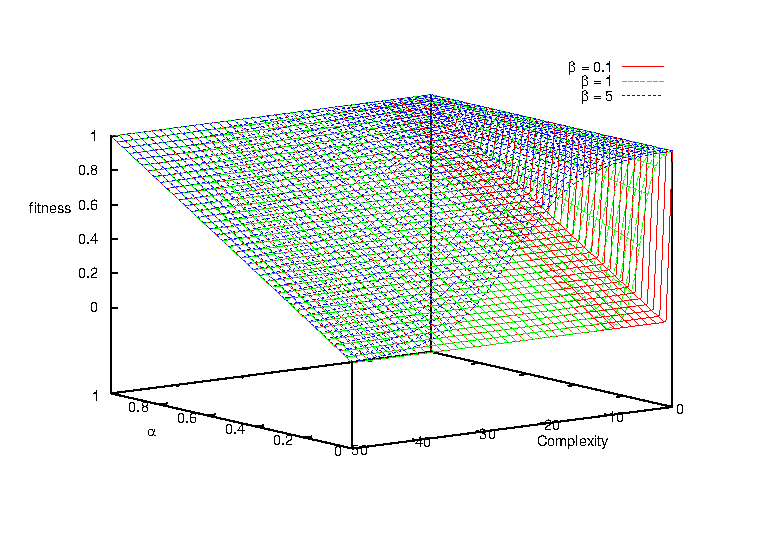
\includegraphics[scale=1.40]{figs/fitness.eps}
  \vspace{-30pt}
  \caption{Поверхности функции $Q_f$ для некоторых $\beta$
    и фиксированного $\tau = 5$.}
  \label{fig:fitness_surph}
\end{figure}

Таким образом, чем лучше результаты суперпозиции и чем она проще, тем ближе значение ее
приспособленности к~$1$.

\begin{algo}
  \label{algo:SA}
  Итеративный алгоритм стохастического порождения суперпозиций.

  Вход:
  \begin{itemize}
	\item Множество порождающих функций $G$, состоящее только из унарных
	  и бинарных функций.
	\item Регрессионная выборка $D$.
	\item $N_{max}$~--- максимальное число одновременно рассматриваемых
	  суперпозиций.
	\item $I_{max}$~--- максимальное число итераций алгоритма.
	\item $\gamma_{mut}$~--- доля суперпозиций, подверженных случайной
	  замене узлов их деревьев.
	\item $\gamma_{cross}$~--- доля суперпозиций, для которых выполняется
	  случайный обмен поддеревьями.
	\item Прочие параметры, используемые в \eqref{eq:q_f} и алгоритме
	  \ref{algo:RF}.
  \end{itemize}
\end{algo}

\begin{enumerate}
  \item Инициализируется упорядоченный набор $\mathcal{X}_f$ суперпозиций.
	А именно, порождается $N_{max}$ суперпозиций алгоритмом $\ref{algo:RF}$.
  \item Оптимизируются параметры $\boldsymbol{\omega}$ суперпозиций
	из $\mathcal{X}_f$ алгоритмом Левенберга-Марквардта.
  \item Выполняются простейшие преобразования, упрощающие суперпозицию:
	например, выражения вида $0 \cdot x$ заменяются на $0$.
  \item Вычисляется значение $Q_f$ для каждой еще не оцененной суперпозиции
	$f$ из $\mathcal{X}_f$: для нее рассчитывается значение функционала качества
	$S_f$ на выборке $D$, и~ставится
	в~соответствие значение $Q_f$ в соответствии с \eqref{eq:q_f}. Для
	суперпозиций, при вычислении $Q_f$ которых была хотя бы раз получена
	ошибка вычислений из-за несовпадения областей определений и значений,
	принимается $Q_f = -\infty$.
  \item Набор суперпозиций $\mathcal{X}_f$ сортируется согласно их
	приспособленности.
  \item Наименее приспособленные суперпозиции удаляются из массива
	$\mathcal{X}_f$ до тех пор, пока его размер не станет равен $N_{max}$.
  \item Отбирается некоторая часть $\gamma_{mut}$ наименее приспособленных
	суперпозиций из $\mathcal{X}_f$. У этой части происходит случайная замена
	одной функции или свободной переменной на другую: генерируются две случайные величины,
	одна из которых служит для выбора вершины дерева $\Gamma_f$, которую
	предстоит изменить, а другая~--- для выбора нового элемента для этой вершины.
	Замена такова, чтобы сохранилась структура суперпозиции, а именно:
	в~случае замены функции сохраняется арность, а свободная переменная
	заменяется только на другую свободную переменную. Исходные
	суперпозиции сохраняются в~массиве $\mathcal{X}_f$.
  \item Повторяются шаги $4-5$.
  \item Производится случайный обмен поддеревьями у $\gamma_{cross}$ наиболее
	приспособленных суперпозиций. Вершины, соответствующие этим поддеревьям,
	выбираются случайным образом. При этом исходные суперпозиции сохраняются
	в~$\mathcal{X}_f$.
  \item Повторяются шаги $2-5$.
  \item Проверяются условия останова: если либо число итераций больше
	$I_{max}$, либо в~массиве $\mathcal{X}_f$ есть хотя бы одна суперпозиция с
	приспособленностью больше, чем $\hat{Q}$, то алгоритм останавливается,
	и результатом является наиболее приспособленная суперпозиция, иначе
	осуществляется переход к~шагу $2$.
\end{enumerate}

\section{Алгоритм преобразования суперпозиций по правилам}

Введем несколько определений.

\begin{defin}
  \label{def:tree_equiv}
  Два дерева $\Gamma_1$ и $\Gamma_2$ равны тогда и только тогда, когда они имеют
  одинаковую структуру и при любой упорядоченной нумерации вершин содержимое
  вершин с одинаковым номером совпадает.
\end{defin}

\begin{defin}
  \label{def:tree_subtree}
  Дерево $\Gamma$ является поддеревом дерева $\Gamma'$, если $\Gamma'$ содержит поддерево,
  равное $\Gamma$ в смысле определения \ref{def:tree_equiv}.
\end{defin}
Такое определение позволяет считать, что дерево является поддеревом другого
дерева, даже если множества вершин этих деревьев не пересекаются.

Напомним, что $f_{V_i}$ обозначает суперпозицию, эквивалентную поддереву вершины
$V_i$.

\begin{defin}
  \label{def:common_comp}
  Общая компонента дерева~--- поддерево $\Delta_{f'}$ дерева $\Gamma_f$ суперпозиции $f$,
  встречающееся более чем один раз.
\end{defin}
Здесь $f'$~--- подвыражение в суперпозици $f$, соответствующее дереву
$\Delta_{f'}$.

Так как суперпозиция $f$ и ее дерево $\Gamma_f$ эквивалентны, общей компонентой
дерева также можно называть суперпозицию, эквивалентную поддереву, являющемуся
общей компонентой в смысле определения \ref{def:common_comp}.

Например, для суперпозиции $(x+2)+(x+2)+x$ общие компоненты: $x$, $2$, $x+2$.

\begin{defin}
  \label{def:max_common_comp}
  Наибольшая общая компонента дерева~--- такая общая компонента $\hat{\Delta}_{f'}$, что не
  существует другой общей компоненты, включающей данную.
\end{defin}
Для вышеупомянутой суперпозиции $(x+2)+(x+2)+x$ наибольшей общей компонентой
является поддерево, соответствующее суперпозиции $x+2$.

Наибольших общих компонент может быть несколько. Например, для суперпозиции
$(x+2) + (x+2) + 2 \sin (x + y) \cos (x + y)$ наибольшими общими компонентами
будут подвыражения $x + 2$ и $x + y$. Обозначим множество всех наибольших общих
компонент графа $\Gamma_f$ суперпозиции $f$ как $\tilde{\Delta}_f$.

Введем также понятие унифицированного графа суперпозиции $f$:
\begin{defin}
  Унифицированный граф $\hat{\Gamma}_f$ суперпозиции $f$~--- направленный
  ациклический граф, полученный из дерева $\Gamma_f$ следующим итеративным 
  методом:
  \begin{enumerate}
	\item Граф $\tilde{\Gamma}_f$ на первом шаге равен $\Gamma_f$.
	\item Для графа $\tilde{\Gamma}_f$ находятся все наибольшие общие компоненты
	  $\hat{\Delta}_{f'}$.
	\item Если таких компонент не найдено, то полученный граф $\tilde{\Gamma}_f$
	  объявляется искомым графом $\hat{\Gamma}_f$, и алгоритм завершается.
	\item Иначе выбирается компонента $\hat{\Delta}_{f'}$ с наибольшей
	  сложностью $C(f')$. Если несколько наибольших общих компонент имеют
	  максимальную сложность, то выбирается первая из них согласно некоторому
	  фиксированному порядку на множестве суперпозиций.
	\item Выбранная компонента остается в единственном экземпляре: удаляются
	  все вершины $V_i$ такие, что $f_{V_i} = f'$, кроме одной вершины $V'_i$,
	  и ребра, входящие в удаленные вершины, изменяются таким образом, чтобы
	  они входили в $V'_i$.
  \end{enumerate}
\end{defin}
То есть, в графе $\hat{\Gamma}_f$ каждая наибольшая общая компонента
$\hat{\Delta}_{f'}$ присутствует не более одного раза.

Таким образом, $\hat{\Gamma}_f$ отличается от $\Gamma_f$ тем, что в одну
вершину могут входить несколько ребер, причем в том и только в том случае,
если эта вершина соответствует поддереву, являющемуся некоторой наибольшей общей
компонентой дерева $\Gamma_f$.

\begin{theorem}
  Граф $\hat{\Gamma}_f$ по данному дереву $\Gamma_f$ строится единственным образом.
\end{theorem}
\begin{Proof}
  Утверждение напрямую следует из метода построения $\hat{\Gamma}_f$,
  если учесть, что не важно, какая именно вершина не была удалена на шаге 5,
  так как после указанного преобразования графа все такие вершины равнозначны.
\end{Proof}

\begin{theorem}
  Дерево $\Gamma_f$ по данному графу $\hat{\Gamma}_f$ восстанавливается единственным образом.
\end{theorem}
\begin{Proof}
  Для того, чтобы построить дерево $\Gamma_f$ по данному графу $\hat{\Gamma}_f$,
  достаточно найти в $\hat{\Gamma}_f$ все вершины $V_i$, имеющие более одной
  родительской вершины $V_j$. Каждой такой вершине $V_i$ соответствует некоторая
  суперпозиция $f_{V_i}$ и ее подграф $\Gamma_f^i$.
  
  Добавим в граф $\Gamma_f$
  такое минимальное число подграфов, равных $\Gamma_f^i$, чтобы каждая вершина
  из $V_j$ указывала в свой собственный подграф, равный $\Gamma_f^i$, то есть,
  чтобы множества вершин дочерних подграфов не пересекались.

  Так как $\hat{\Gamma}_f$ построен путем выделения и объединения общих компонент
  дерева $\Gamma_f$, то полученный в результате указанной процедуры граф будет
  являться деревом, причем, эквивалентным $\Gamma_f$.
\end{Proof}

Из этих двух утверждений непоследственно следует следующая теорема:
\begin{theorem}
  Между $\hat{\Gamma}_f$ и $\Gamma_f$ существует взаимно однозначное преобразование.
\end{theorem}

Эта теорема позволяет говорить об эквивалентности $\Gamma_f$ и $\hat{\Gamma}_f$
и о том, что взаимно однозначные преобразования для $\hat{\Gamma}_f$ являются
также и взаимно однозначными преобразованиями для суперпозиции $f$.

Работа алгоритма преобразования суперпозиций по правилам состоит из двух этапов.
\begin{enumerate}
  \item Находятся наибольшие равные в смысле определения \ref{def:tree_equiv}
	поддеревья, и дерево $\Gamma_f$ суперпозиции $f$ преобразуется в
	соответствующий унифицированный граф $\hat{\Gamma}_f$.
  \item К полученному графу $\hat{\Gamma}_f$ применяются правила преобразования,
	уменьшающие его сложность, до тех пор, пока правила возможно применять.
\end{enumerate}

Опишем эти этапы в следующих двух разделах.

\subsection{Алгоритм выделения наибольших общих компонент дерева}

Введем понятие пути $\text{PathTo}$ до вершины $V_i$. Пусть дана некоторая
лексикографическая нумерация вершин дерева $\Gamma_f$ суперпозиции $f$. Тогда
путь из корня дерева $V_0$ до вершины $V_i$~--- последовательность номеров
вершин в соответствующем пути из корня в $V_i$. Будем обозначать эту
последовательность как $\text{PathTo} (V_i)$.

Рассмотрим некоторую суперпозицию $f'$, являющуюся подвыражением суперпозиции
$f$, и пусть суперпозиции $f'$ соответствуют вершины
$V_{i_1}, V_{i_2}, \dots, V_{i_k}$. Будем обозначать множество путей в
соответствующие $f'$ вершины как $\mathbf{Paths}(f')$. То есть,
\[
\mathbf{Paths}(f') = \{ \text{PathTo} (V_i) \mid f_{V_i} = f' \}.
\]

Опишем алгоритм выделения наибольших общих компонент $\hat{\Delta}_{f'}$.
\begin{algo}
  \label{algo:BCCIsolator}
  Алгоритм выделения наибольших общих компонент графа $\Gamma_f$.
\end{algo}
\begin{enumerate}
  \item Пронумеруем вершины $V_i \mid i \in \{1, \dots, C(f)\}$ в
	лексикографическом порядке.
  \item Построим функцию $\text{NTS}$ (анг. Node To Superposition), сопоставив каждой
	вершине $V_i$ суперпозицию, имеющую корнем $V_i$:
	\[
	\text{NTS} : V_i \mapsto f_{V_i} \in \mathcal{F}_{\Gamma_f} \subset \mathcal{F},
	\]
	где $\mathcal{F}_{\Gamma_f}$~--- множество всех суперпозиций, являющихся
	подвыражениями суперпозиции $f$.

	Заметим, что функция $\text{NTS}$, сюръективна по построению, но она не является инъективной:
	могут существовать такие $i \neq j$, что $\text{NTS} (V_i) = \text{NTS} (V_j)$.
  \item Для каждой суперпозиции $f_{V_i}$ из множества значений $\text{NTS}$ добавим
	путь к каждой из вершин, соответствующей $f_{V_i}$, в список путей для
	суперпозиции $f_{V_i}$.

	Таким образом, мы получили функцию $\text{STP}$ (анг. Superposition To
	Paths), сопоставляющую каждой суперпозиции $f'$, являющейся подвыражением
	суперпозиции $f$, путь $\text{PathTo}$ до вершин $V_i$, ей соответствующих:
	\[
	\text{STP} : f_{V_i} \mapsto \mathbf{Paths}(f_{V_i}) = \{ \text{PathTo}(V_i) \mid \text{NTS} (V_i) = f_{V_i} \}.
	\]
  \item Расположим суперпозиции $f_{V_i}$ по возрастанию соответствующей длины
	пути в $\text{STP}(f_{V_i})$, и для каждой суперпозиции, встречаемой по меньшей мере два
	раза, найдем и удалим все прочие суперпозиции, у которых пути получаются
	приписыванием одинакового числа номеров вершин к соответствующему пути.
\end{enumerate}

Построенный алгоритм позволяет найти в суперпозиции подвыражения,
встречающиеся более одного раза. При этом алгоритм позволяет не рассматривать
многократно встречающиеся суперпозиции, являющиеся подвыражениями других
суперпозиций.

\subsection{Применение правил преобразования унифицированных графов выражения}

Определим понятие правила $\mathbf{R}$ преобразования графа следующим образом:
\begin{defin}
  \label{def:rewriting_rule}
  Правило $\mathbf{R}$ преобразования графа~--- пара $(L, R)$, где $L$ обозначает граф-шаблон,
  а $R$~--- граф-замену.
\end{defin}
Преобразование графа $\Gamma$ по правилу $\mathbf{R}$ сводится к поиску
изоморфного $L$ графа в $\Gamma$ и его замене на граф $R$.

Обозначим $\mathcal{R} = \{\mathbf{R}\}$ множество правил преобразования графа.

Рассмотримчастные случаи определения \ref{def:rewriting_rule}, возникающие при работе с
унифицированными графами $\hat{\Gamma}_f$. Будем считать, что множество
элементарных функций $G$ состоит только из функций одного и двух аргументов.

\paragraph{Функции одного аргумента.} Ограничимся рассмотрением правил вида
\begin{equation}
  \label{eq:unary_rule}
  \mathbf{R} = (L, R) = (g_i, g_j) = (g_{i_1} \circ g_{i_2} \circ \dots \circ g_{i_n}, g_{j_1} \circ g_{j_2} \circ \dots \circ g_{j_m}) \mid n > m.
\end{equation}
Иными словами, мы рассматриваем правила, заменяющие суперпозицию $n$ функций
одного аргумента на суперпозицию меньшего числа функций одного аргумента. То
есть, рассматриваются правила, где сложность графа-шаблона $L$ больше, чем
сложность графа-замены $R$: $C(L) = C(g_i) > C(R) = C(g_j)$.

Приведем примеры таких правил:
\begin{itemize}
  \item $(\arcsin \circ \sin, \text{id}),$
  \item $(\log \circ \exp, \text{id}).$
\end{itemize}

Применение правил вида \eqref{eq:unary_rule} к графу $\hat{\Gamma}_f$ суперпозиции
$f$ сводится к поиску вершин, соответствующих функциям из $L$,
и замене всех найденных вхождений на правую часть правила $R$. То есть, для
каждого правила $\mathbf{R} = (L, R)$ в графе $\hat{\Gamma}_f$ ищется
суперпозиция, соответствующая суперпозиции, описываемой графом-шаблоном $L$,
и каждое найденное вхождение заменяется на суперпозицию, описываемую
графом-заменой $R$.

\paragraph{Функции двух аргументов.} Заметим, что используемые графы-шаблоны
в этом случае представимы в виде тройки $L = (Lst, Rst, Op)$, где $Op$~--- бинарная операция,
дочерними подграфами которой являются подграфы $Lst$ и $Rst$. Граф-замена $R$
является функцией от двух аргументов: $R = R (Lst, Rst)$. Эта функция возвращает
граф-замену, соответствующий подграфам $Lst$ и $Rst$, найденным в графе $\Gamma_f$.

Введем понятие переменной на множестве графов.
\begin{defin}
  Переменная $t_i$ на множестве графов $\Gamma$ в графе $\hat{\Gamma}_f$~---
  вершина $V_j, j = j(t_i)$ в графе $\hat{\Gamma}_f$. Подстановка некоторого
  значения $t_i = \Gamma_0$ в граф $\hat{\Gamma}_f$ эквивалентна замене вершины
  $t$ на граф $\Gamma_0$.
\end{defin}
Говоря о графе суперпозиции $f$ с переменной $t_i$, будем иметь ввиду любой
граф, получаемый заменой $t_i$ на произвольный подграф. Так, $\cos^2 t_i$
является графом суперпозиции $\cos^2 (x + 2)$ при $t_i = (x + 2)$.

$Lst$ и $Rst$ являются шаблонами графов~--- это графы, содержащие
некоторый набор переменных $t_i$. Таким образом, поиск подграфа $Lst_{\Gamma_f}$
в графе $\Gamma_f$, соответствующего $Lst$, сводится к поиску таких значений
переменных $t_i$, входящих в $Lst$, при которых граф $Lst$ становится равен
графу $Lst_{\Gamma_f}$. Аналогично происходит поиск подграфа, соответствующего
$Rst$.

Учитывая, что для каждой тройки $(Lst, Rst, Op)$ задается своя функция $R$, можно
сказать, что функция $R$ на самом деле является функцией от всех входящих в $Lst$
и $Rst$ переменных: $R = R (\{t_i\}, \{t_j\})$, где $\{t_i\}$~--- переменные,
входящие в состав графа $Lst$, а $\{t_j\}$~--- переменные, входящие в состав
графа $Rst$.

Если $Op$ коммутативна, то $Lst$ и $Rst$ можно поменять местами. Если $Op$ ассоциативна,
то правило применимо не только к суперпозициям, соответствующим выражениям вида
$Op (Lst, Rst)$, но и выражениям вида $Op (Lst, Op (Rst, t))$, где $t$~--- некоторый
не участвующий в правиле подграф. В таком случае выражение вида $Op (Lst, Op (Rst, t))$
заменяется на $Op (R (Lst, Rst), t))$.

Приведем процедуру поиска соответствий для случая неассоциативной и
некоммутативной $Op$.
\begin{enumerate}
  \item В графе суперпозиции находятся все вершины $V_i$, содержащие $Op$.
  \item Если существует набор значений переменных $t_l$, используемых в $Lst$,
	при подстановке которых в $Lst$ граф $Lst$ становится равен первому (по
	порядку) дочернему подграфу вершины $V_i$ (то есть, первому аргументу
	функции в вершине $V_i$), то считается, что первый аргумент $V_i$
	соответствует шаблону, заданному $Lst$.
  \item Аналогично проверяется, соответствует ли шаблону $Rst$ второй аргумент
	функции в вершине $V_i$.
  \item Если оба аргумента соответствуют шаблонам, и при этом значения
	переменных $t$ с одинаковыми индексами равны, то считается, что подграф,
	соответствующий вершине $V_i$, подходит под правило $(Lst, Rst, Op)$.
\end{enumerate}
Случай коммутативной операции $Op$ сводится к случаю некоммутативной неявным добавлением
правил $(Rst, Lst, Op)$ для каждого $(Lst, Rst, Op)$.
Случай ассоциативной операции $Op$ аналогичен случаю неассоциативной, но с добавлением
перебора по всем возможным комбинациям пар аргументов.

После нахождения соответствия участка графа правилу $((Lst, Rst, Op), R)$ соответствующие
значения переменных, полученные в шагах $2-3$, подставляются в функцию $R$, и исходно
найденное подвыражение заменяется на значение этой функции.

Унифицированный граф суперпозиции используется для того, чтобы избежать сравнений подграфов
в шаге $4$. Вместо этого проверяется, соответствуют ли одинаковые переменные одному и тому
же подграфу в унифицированном графе суперпозиции.

Рассмотрим для примера правило, описывающее основное тригонометрическое
тождество $\sin^2 x + \cos^2 x = 1$. В этом случае $Op$~ соответствует $+$, а
$Lst$ и $Rst$ представлены на рис. \ref{fig:lst_example} и \ref{fig:rst_example}
соответственно. Функция $R = R(t)$ возвращает граф из единственного узла $1$.

\begin{figure}[h]
  \centering
  \begin{tikzpicture}
	\scalefont{4}
	\tikzstyle{n} = [draw, inner sep=2pt, fill=red!20]
	  \begin{dot2tex}[dot,options=-tmath,scale=0.4]
		digraph G1 {
		  node [shape="circle",style="n"];
		  
		  Pow [label="pow"];
		  Sin [label="\sin"];
		  C2 [label="2"];
		  t [label="t_1"];

		  Pow -> Sin;
		  Pow -> C2;
		  Sin -> t;
		}
	  \end{dot2tex}
	\end{tikzpicture}
  \caption{Представление $Lst$ для правила $\sin^2 x + \cos^2 x = 1$.}
  \label{fig:lst_example}
\end{figure}

\begin{figure}[h]
  \centering
  \begin{tikzpicture}
	\scalefont{4}
	\tikzstyle{n} = [draw, inner sep=2pt, fill=red!20]
	  \begin{dot2tex}[dot,options=-tmath,scale=0.4]
		digraph G1 {
		  node [shape="circle",style="n"];
		  
		  Pow [label="pow"];
		  Cos [label="\cos"];
		  C2 [label="2"];
		  t [label="t_1"];

		  Pow -> Cos;
		  Pow -> C2;
		  Cos -> t;
		}
	  \end{dot2tex}
	\end{tikzpicture}
  \caption{Представление $Rst$ для правила $\sin^2 x + \cos^2 x = 1$.}
  \label{fig:rst_example}
\end{figure}

При применении правила к суперпозиции $\cos^2 (x + 2) + \sin^2 (x + 2)$ переменная
$t_1$ примет значение, соответствующее графу суперпозиции $x + 2$, как для $Lst$,
так и для $Rst$, поэтому правило будет успешно применено.

Заметим, что, например, правило, описывающее вынесение общего множителя за
скобки, заменяющее $ax + bx$ на $(a + b)x$, неприменимо к суперпозиции типа
$nx + x$ в описанном выше виде. Это связано с тем, что, например, шаблон $Rst$
у такого правила представляет умножение константы на переменную, в то время
как в суперпозиции $nx + x$ второй аргумент представляет собой просто константу.

Чтобы избежать подобной ситуации, в работе предлагается указывать каждое
подобное соотношение не в виде правил переписывания графа, а в виде отношений
эквивалентности, что позволяет существенно сократить количество указываемых вручную
правил.

\section{Метод исследования стабильности порожденной модели}

Для оценки устойчивости $\mathbb{T}_{\hat{f}}$ решения $\hat{f}$ задачи
\eqref{eq:s_common}, как предложено выше, фиксируется структурный вид суперпозиции
$\hat{f}$ и исследуется зависимость стандартного отклонения ее коэффициентов
как функция стандартного отклонения нормально распределенной случайной добавки
в исходных данных.

Иными словами, выбираются значения $\sigma_{\lambda}$ и $\sigma_n$, затем для этих
значений генерируется выборка $\acute{D}(\sigma_n, \sigma_{\lambda})$ согласно
\eqref{eq:d_acute}. Для этой выборки вычисляются значения коэффициентов суперпозиции
$\hat{f}$, минимизирующие функционал \eqref{eq:s_common} согласно \eqref{eq:hat_omega},
методом Левенберга-Марквардта.

Данная процедура для фиксированной пары $\sigma_{\lambda}$ и $\sigma_n$ повторяется
до достижения некоторого критерия останова (например, по количеству итераций),
после которого и рассчитывается $\mathbb{T}_{\hat{f}}$.

Повторяя описанные выше шаги для различных $\sigma_{\lambda}$ и $\sigma_n$, можно
оценить зависимость стандартного отклонения коэффициентов суперпозиции от
стандартного отклонения шума.

Из физических соображений ясно, что гладкий вид такой зависимости означает устойчивое в
физическом смысле решение, тогда как отклонения от гладкости означают
ту или иную ошибку в суперпозиции и могут являться свидетельством переобучения:
чем меньше коэффициенты зависят от случайных шумов в данных, тем больше обобщающая
способность.

Кроме того, сравнение различных суперпозиций может также производиться по
критерию устойчивости в дополнение к сравнению по сложности и по значению
функционала \eqref{eq:s_common}. В ряде практических приложений критерий устойчивости
может иметь приоритетное значение.

\section{Вычислительный эксперимент}

\subsection{Порождение суперпозиций}

\subsubsection{Синтетические данные}
Восстанавливается функциональная зависимость
$z = 2 \cosh \frac{\sqrt{x^2 + y^2}}{2} \mid x \in [-1; 1], y \in [-1; 1]$,
соответствующая образующей фигуры вращения цепной линии. При этом значения зависимой
переменной $z$ были искусственно зашумлены аддитивной добавкой из
распределения $\mathcal{N} (0, 0.1)$, и соответствующая ей переменная
присутствовала во множестве используемых свободных переменных.
Также был искусственно добавлен один
выброс~--- точка с координатами $(0, 0, -1)$.

В качестве функционала ошибки $S_f$ используется сумма квадратов
регрессионных остатков для данной суперпозиции $f$ с вектором параметров
$\boldsymbol{\omega}$ при регрессионной выборке $D$:
\begin{equation}
  \label{eq:sse_expr}
  S(\boldsymbol{\omega}, f, D) = \sum_{i=1}^N (y_i - f (\boldsymbol{\omega}, \mathbf{x}_i))^2.
\end{equation}

Значение функционала ошибки $S_f$ при подстановке исходной незашумленной
функциональной зависимости составляет $\approx 13.28$, сложность исходной
суперпозиции~--- $16$.

\begin{table}[h]
  \centering
  \caption{Результаты вычислительного эксперимента для предложенного алгоритма.}
  \begin{tabular}{| c | c | l | c | c |} \hline
	$N$ & $i$	& \multicolumn{1}{c|}{Суперпозиция}																										& $S_f$				& $C(f)$ \\ \hline
	1	& 16	& $0.9998 \left(2.71^{\frac{\sqrt{x \cdot x + y^2}}{2.02}} + 2.57^{\frac{\sqrt{x \cdot x + y ^2}}{-1.94}}\right) - 0.0059$				& $\approx 13.25$	& 31	\\ \hline
	2	& 7		& $1.999 \cosh \frac{\sqrt{x \cdot x + y \cdot y \cdot 1.0002}}{2.002}$																	& $\approx 13.89$	& 16	\\ \hline
  \end{tabular}
  \label{tabl:results_synth}
\end{table}

\begin{table}[h]
  \centering
  \caption{Результаты вычислительного эксперимента для алгоритма \cite{Zelinka2008}.}
  \begin{tabular}{| c | c | c | c |} \hline
	$i$ & Суперпозиция																					& $S_f$				& $C(f)$ \\ \hline
	29  & $2.69^{\frac{\sqrt{x \cdot x + y \cdot y}}{2.1}} + \frac{x \cdot x}{6988} + \frac{y}{1896} - \frac{x \cdot y \cdot y}{504} + 0.69 + 0.00079 \cdot x \cdot x \cdot y \cdot y$				& $\approx 25.44$	& 43	\\ \hline
  \end{tabular}
  \label{tabl:results_Z}
\end{table}

Использованные параметры алгоритма \ref{algo:SA}: $N_{max} = 200, I_{max} = 50,
\hat{Q} = 0.95, \tau = 20, \alpha = 0.05$, $\beta = 1$, $\gamma_{mut} = \frac{1}{3}$,
$\gamma_{cross} = \frac{1}{3}$. При отсутствии улучшения результатов в~течение
нескольких итераций подряд алгоритм \ref{algo:SA} также завершался.

Результаты вычислительного эксперимента приведены в таблице \ref{tabl:results_synth}.
Указан номер итерации $i$, на которой суперпозиция была впервые
получена, сама суперпозиция, среднеквадратичная ошибка \eqref{eq:sse_expr} и сложность в
смысле количества узлов в соответствующем графе выражения. Числовые коэффициенты
в приведенных формулах и значения функционала $S_f$ искусственно округлены до
нескольких значащих цифр.

Алгоритм запускался для двух разных наборов элементарных функций.
В обоих случаях элементарные функции включали в себя стандартные арифметические операции и
операцию возведения в степень. Для удобства восприятия возведение в степень
$\frac{1}{2}$ (и близкие ей) представлено в таблице как извлечение корня.

В первом случае в наборе отсутствовала функция $\cosh$. При этом по результатам
10 запусков наилучшей суперпозицией, полученной предложенным алгоритмом,
являлась функция за номером 1 из таблицы \ref{tabl:results}. Видно, что выражение
в скобках близко определению $\cosh x = \frac{e^x + e^{-x}}{2}$,
однако, разные значения оснований степенных функций могут затруднить экспертный
анализ полученного выражения, которое само по себе является достаточно громоздким.

Во втором случае набор элементарных функций также включал в себя функцию
$\cosh$, результату этого выражения соответствует суперпозиция за номером 2.
Включение $\cosh$ в $G$ позволило существенно быстрее подобрать искомую функцию, и сложность
получившейся суперпозиции также существенно меньше.

Кроме того, предложенный алгоритм сравнивался с алгоритмом \cite{Zelinka2008},
где предложено кодировать суперпозицию бинарной строкой и применять стандартные
генетические алгоритмы на бинарных строках. При этом, в множестве используемых
функций также отсутствовала функция $\cosh$.

Наилучшая суперпозиция, полученная алгоритмом \cite{Zelinka2008} по результатам
10 запусков, приведена в таблице \ref{tabl:results_Z}. Полученная суперпозиция
имеет существенно более высокую сложность, чем суперпозиции, перечисленные в
таблице \ref{tabl:results_synth}, что может быть связано с отсутствием этапов упрощения
суперпозиции и отсутствием множителя, соответствующего сложности суперпозиции,
при оценке приспособленности суперпозиции в алгоритме \cite{Zelinka2008}.

\renewcommand{\thesubfigure}{\thefigure}
\makeatletter
  \renewcommand{\p@subfigure}{}
  \renewcommand{\@thesubfigure}{}
\makeatother

\begin{figure}[h]
  \centering
  \subfigure[(а)]{%
	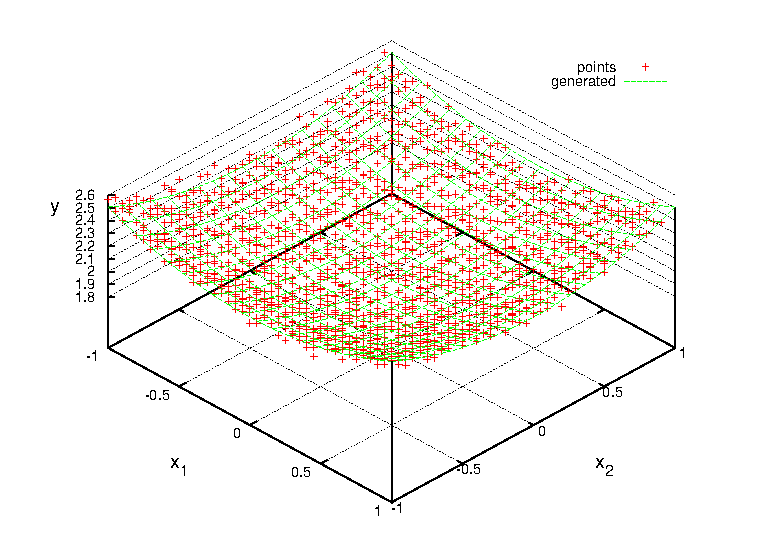
\includegraphics[scale=0.6]{figs/1-data.eps}%
	\label{fig:1_results_data}%
  }%
  \subfigure[(б)]{%
	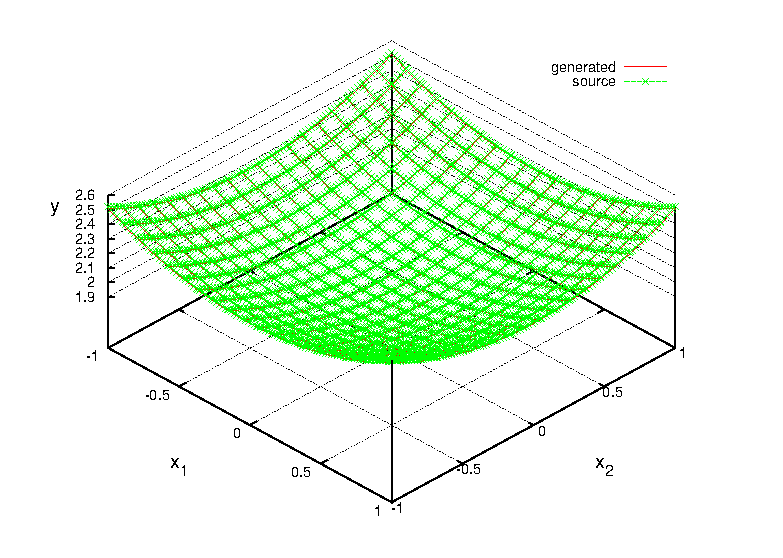
\includegraphics[scale=0.6]{figs/1-source.eps}%
	\label{fig:1_results_source}%
  }
  \caption{Первая порожденная суперпозиция и зашумленные точки выборки (a) и исходная зависимость (б).}
  \label{fig:1_results}
\end{figure}

\begin{figure}[h]
  \centering
  \subfigure[(а)]{%
	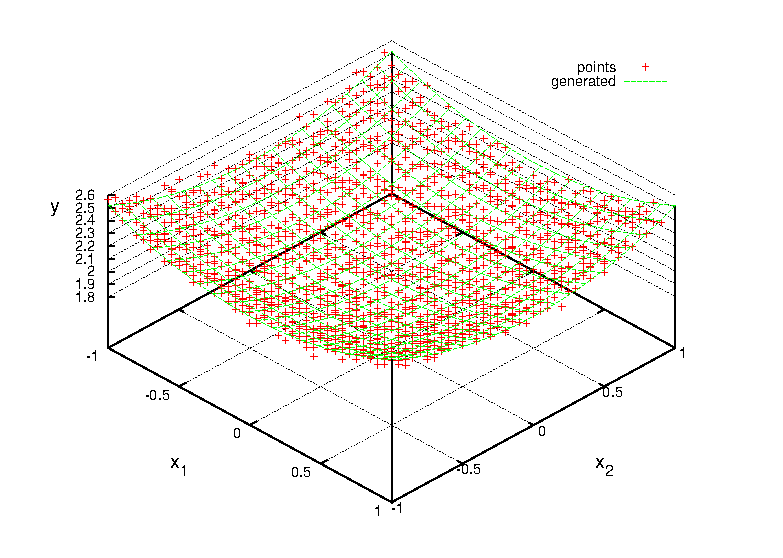
\includegraphics[scale=0.6]{figs/2-data.eps}%
	\label{fig:2_results_data}%
  }%
  \subfigure[(б)]{%
	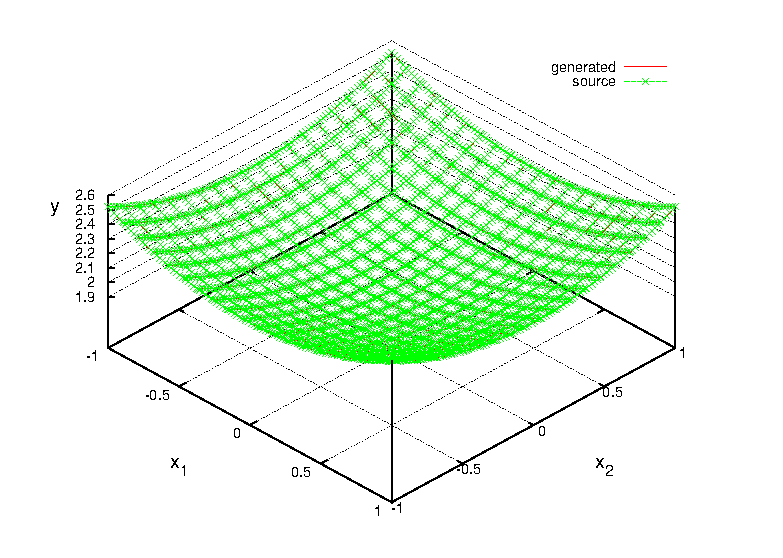
\includegraphics[scale=0.6]{figs/2-source.eps}%
	\label{fig:2_results_source}%
  }
  \caption{Вторая порожденная суперпозиция и зашумленные точки выборки (a) и исходная зависимость (б).}
  \label{fig:2_results}
\end{figure}

На рис. \ref{fig:1_results} отображены изометрические
проекции первой из приведенных в таблице \ref{tabl:results_synth} суперпозиций. На
графике слева данная суперпозиция сравнивается с точками синтезированной
зашумленной выборки, на графике справа она же приведена вместе
с исходной незашумленной зависимостью. Аналогичные проекции
приведены для второй суперпозиции на рис. \ref{fig:2_results}.

\subsubsection{Моделирование волатильности опционов}

Восстанавливается регрессионая зависимость
волатильности опциона от его стоимости и сроков исполнения
\cite{daglish07theory,strijov09jct}. Используются исторические данные о
волатильности опционов Brent Crude Oil. Срок действия опциона~--- полгода,
с 02.01.2001 по 26.06.2001, тип~--- право на продажу базового инструмента.
Базовым инструментом в~данном случае является нефть. Использовались
ежедневные цены закрытия опциона и~базового инструмета.

Данный инструмент имеет низкую волатильность, вследствие чего среди данных
нет выбросов. В~данных имеются пропуски, так как опционы с ценами, далекими
от цен базового инструмента, не торговались сразу после выпуска опционов.

\begin{table}[h]
  \centering
  \begin{tabular}{| c | c | c | c |} \hline
	$i$ & Суперпозиция													& $S_f$				& $C(f)$ \\ \hline
	9	& $\displaystyle \left(\frac{1.36}{xy}\right)^{0.48}$			& $\approx 0.0182$	& 7		\\ \hline
	14	& $\displaystyle (15.8y + \arcsin y)^{-0.48}$					& $\approx 0.0208$	& 8		\\ \hline
	13	& $\displaystyle (yx^{0.882} + \arcsin y)^{-0.482}$				& $\approx 0.0178$	& 10	\\ \hline
	8	& $\displaystyle 0.125 \frac{y}{(y^2)^{0.8+y}}$					& $\approx 0.0171$	& 11	\\ \hline
	14	& $\displaystyle \frac{\frac{3.86 \cdot 10^{11} + y}{\frac{y\frac{1.227 \cdot 10^{11}}{x^y}-2.46 \cdot 10^{8}}{y \cos \left(\frac{\frac{-5.89 \cdot 10^{-3}+y}{\frac{y - 5.47 \cdot 10^{-3}}{y \cos y}}}{y}\right)}}}{y^y \cos y + xy}$	& $\approx 0.0092$	& 42		\\ \hline
  \end{tabular}
  \caption{Результаты вычислительного эксперимента}
  \label{tabl:results}
\end{table}

\begin{table}
  \centering
  \begin{tabular}{c c}
	\begin{tikzpicture}
	  \scalefont{4}
	  \tikzstyle{n} = [draw, inner sep=4pt, fill=red!20]
	  \begin{dot2tex}[dot,options=-tmath,scale=0.4]
		digraph G1 {
		  node [shape="circle",style="n"];
		  
		  Pow [label="\bullet ^ \bullet"];
		  Div [label="\div"];
		  Mul [label="\bullet \times \bullet"];
		  X [label="$x$"];
		  Y [label="$y$"];
		  C1 [label="0.48"];
		  C2 [label="1.36"];

		  Pow -> Div;
		  Pow -> C1;

		  Div -> C2;
		  Div -> Mul;

		  Mul -> X;
		  Mul -> Y;
		}
	  \end{dot2tex}
	\end{tikzpicture} & \begin{tikzpicture}
	  \scalefont{4}
	  \tikzstyle{n} = [draw, inner sep=4pt, fill=red!20]
	  \begin{dot2tex}[dot,options=-tmath,scale=0.4]
		digraph G3 {
		  node [shape="circle",style="n"];
		  
		  Pow [label="\bullet ^ \bullet"];
		  Plus [label="\bullet + \bullet"];
		  Mul [label="\bullet \times \bullet"];
		  C1 [label="15.8"];
		  Y1 [label="$y$"];
		  Asin [label="\arcsin"];
		  Y2 [label="$y$"];
		  C2 [label="-0.48"];

		  Pow -> Plus;
		  Pow -> C2;

		  Plus -> Mul;
		  Plus -> Asin;

		  Mul -> Y1;
		  Mul -> C1;

		  Asin -> Y2;
		}
	  \end{dot2tex}
	\end{tikzpicture} \\
	Граф суперпозиции $\left(\frac{1.36}{xy}\right)^{0.48}$ & Граф суперпозиции $(15.8y + \arcsin y)^{-0.48}$
  \end{tabular}
  \caption{Графы результирующих суперпозиций}
  \label{fig:expr_tree_res}
\end{table}

В ходе предварительной обработки данных выяснено, что для больших значений волатильности
зависимость принимает существенно неоднозначный характер, поэтому для облегчения
аналитического описания моделировалась зависимость цены от волатильности
и~времени.

Использованные параметры алгоритма \ref{algo:SA}: $N_{max} = 200, I_{max} = 50,
\hat{Q} = 0.95, \tau = 10, \alpha = 0.05$, $\gamma_{mut} = \frac{1}{3}$,
$\gamma_{cross} = \frac{1}{3}$. При отсутствии улучшения результатов в~течение
нескольких итераций подряд алгоритм \ref{algo:SA} также завершался.

В таблице \ref{tabl:results} приведены некоторые из суперпозиций,
порожденных в результате работы алгоритма \ref{algo:SA}, в порядке возрастания
их сложности. Указан номер итерации $i$, на которой суперпозиция была впервые
получена, сама суперпозиция, среднеквадратичная ошибка ($S_f$) и сложность в
смысле количества узлов в соответствующем графе выражения. Числовые коэффициенты
в приведенных формулах и значения функционала $S_f$ искусственно округлены до
$2-3$ значащих цифр. Переменная $x$ в суперпозициях обозначает срок исполнения
опциона, $y$~--- волатильность.


\begin{figure}[h]
  \centering
  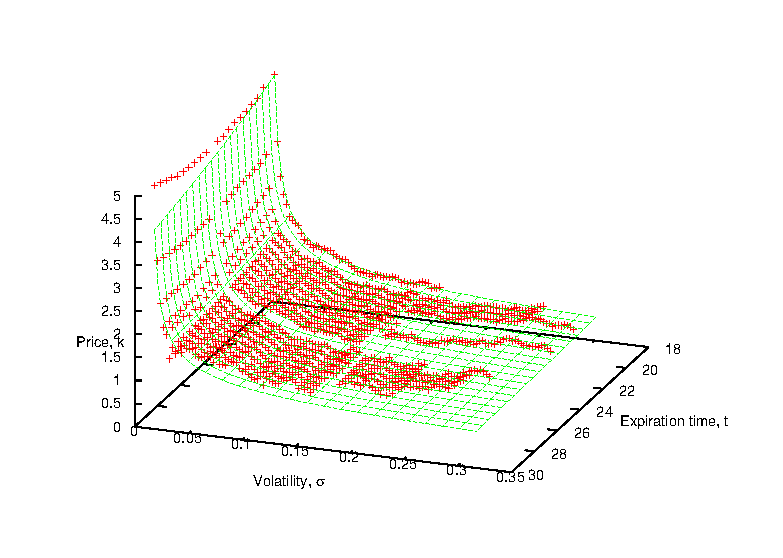
\includegraphics[scale=1.1]{figs/1-iso.eps}
  \caption{Изометрическая проекция результирующей суперпозиции}
  \label{fig:1_iso}
\end{figure}

\begin{figure}[h]
  \centering
  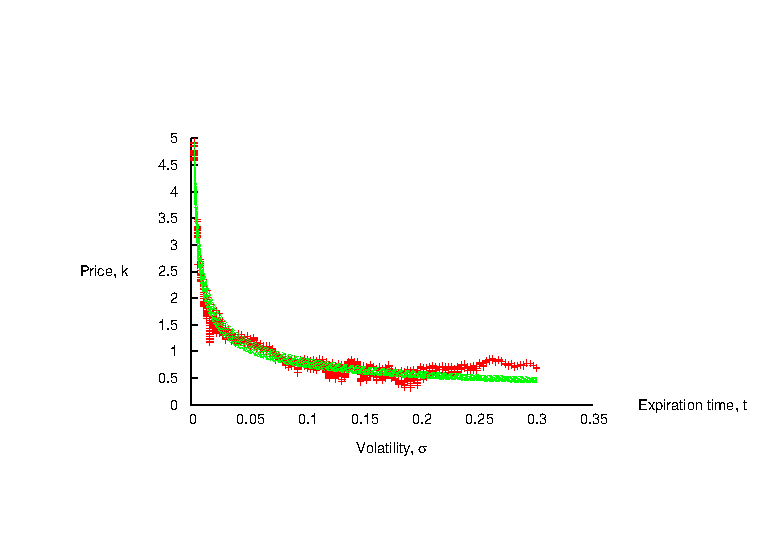
\includegraphics[scale=1.1]{figs/1-proj.eps}
  \caption{Проекция результирующей суперпозиции на плоскость $(\sigma, k)$}
  \label{fig:1_proj}
\end{figure}

В таблице $\ref{fig:expr_tree_res}$ представлены графы
первых двух упомянутых в таблице суперпозиций. На рисунках \ref{fig:1_iso} и
\ref{fig:1_proj} отображены изометрическая проекция и проекция на одну из
плоскостей для суперпозиции $\left(\frac{1.36}{xy}\right)^{0.48}$. 

\subsection{Упрощение суперпозиций}
\newcommand{\NBin}[1]{\mathbf{NBin}\ \text{#1}\ }
\newcommand{\NUn}[1]{\mathbf{NUn}\ \text{#1}\ }
\newcommand{\LVar}{\mathbf{LVar}\ }
\newcommand{\LC}{\mathbf{LC}\ }

В вычислительном эксперименте предложенный алгоритм применяется к
суперпозициям, сгенерированным вручную.

Результаты применения предложенного алгоритма также сравниваются с
результатами, полученными применением программы GNU Octave с пакетом Symbolic
\cite{SymbolicPackage} к тем же выражениям. Пакет Symbolic основан на системе
символьных вычислений GiNaC \cite{GinacSite}.

Суперпозиции вместе с результатами
перечислены в таблице \ref{tabl:results_1}. Исходным суперпозициям соответствует
колонка $f$, полученным в результате применения предложенного алгоритма
суперпозициям соответствует колонка $\hat{f}$, а суперпозициям, полученным в
результате применения GNU Octave~--- $f_{oct}$. Если суперпозиция не была
упрощена, на соответствующем месте ставится прочерк.

При описании правил будем пользоваться следующими обозначениями для вершин
различного типа:
\begin{itemize}
  \item $\NBin{Op} t1\ t2$ обозначает вершину $V_i$ с функцией $\text{Op}$ от двух
	аргументов~--- $t1$ и $t2$.
  \item $\NUn{Op} t$ обозначает вершину $V_i$ с функцией $\text{Op}$ ОТ одного
	аргумента $t$.
  \item $\LVar x_i$ обозначает вершину $V_i$ с переменной $x_i$.
  \item $\LC c$ обозначает вершину $V_i$ с константой $c$.
\end{itemize}

Перечислим используемые элементарные функции одного аргумента из $G$:
\[
\text{Sin, Cos, Log, Tan, Asin, Acos, Atan, Id.}
\]

Используются следующие обозначения для функций двух переменных из $G$:
\begin{itemize}
  \item $\text{Plus, Minus, Mul, Div}$: операции сложения, вычитания, умножения и
	деления соответственно.
  \item $\text{Pow}$: операция возведения в степень. Первый ее аргумент возводится в
	степень, соответствующую второму.
\end{itemize}

Используемый набор правил для функций двух аргументов включал в себя, в том числе,
следующие нетривиальные правила:
\begin{enumerate}
  \item Функция от двух констант заменяется на соответствующее значение этой функции.
	\[
	(f, \LC a, \LC b) \mapsto \LC f (a, b).
	\]
  \item Дистрибутивность умножения:
	\[
	(\text{Plus}, \NBin{Mul} (\LC a)\ t, \NBin{Mul} (\LC b)\ t) \mapsto \NBin{Mul} (\LC (a + b))\ t.
	\]
  \item Внесение константы под знак деления:
	\[
	(\text{Mul}, \LC a, \NBin{Div} t\ (\LC b)) \mapsto \NBin{Div} t\ (\LC \frac{a}{b}).
	\]
  \item Сворачивание выражений вида $at^2 + bt$ в квадрат суммы:
	\begin{align}
	  (\text{Plus}, &\NBin{Mul} (\LC a)\ (\NBin{Pow} t\ (\LC 2)), \NBin{Mul} (\LC b)\ t) \mapsto \nonumber\\
		\mapsto &\NBin{Plus}\nonumber\\
				&\ \ \ \ \ \ (\NBin{Pow} (\NBin{Plus} (\NBin{Mul} (\LC \sqrt a)\ t)\ (\LC \frac{b}{2 \sqrt a}))\ (\LC 2))\nonumber\\
				&\ \ \ \ \ \ (\LC (-(\frac{b}{2 \sqrt a})^2)).\nonumber
	\end{align}
  \item Произведение и частное степеней:
	\[
	(\text{Mul}, \NBin{Pow} t\ (\LC a), \NBin{Pow} t\ (\LC b)) \mapsto \NBin{Pow} t\ (\LC (a + b)),
	\]
	\[
	(\text{Div}, \NBin{Pow} t\ (\LC a), \NBin{Pow} t\ (\LC b)) \mapsto \NBin{Pow} t\ (\LC (a - b)).
	\]
  \item Формула двойного угла:
	\[
	(\text{Mul}, \NUn{Cos} t, \NUn{Sin} t) \mapsto \NBin{Div} (\NUn{Sin} (\NBin{Mul} (\LC 2)\ t))\ (\LC 2)
	\]
  \item Последовательное возведение в степень ${t^a}^b$:
	\[
	(\text{Pow}, \NBin{Pow} t\ (\LC a), \LC b) \mapsto \NBin{Pow} t\ (\LC ab).
	\]
\end{enumerate}

Следующие деревья принимаются изоморфными:
\begin{enumerate}
  \item $\NBin{Minus} t\ (\LC b) \equiv \NBin{Plus} t\ (\LC (-b))$
  \item $t \equiv \NBin{Mul} (\LC 1)\ t \equiv \NBin{Pow} t\ (\LC 1)$
\end{enumerate}

Также при упрощении подвыражения вида $\NUn{g} (\LC c)$ заменяются на $\LC (g (c))$,
то есть, функции одного аргумента от константы заменяются на значение
соответствующих функций при подстановке этой константы. Данная подстановка
выполняется рекурсивно: например, выражение $\tan \sin 0$ заменится на
константу $0$.

\begin{table}[h]
  \centering
  \begin{tabular}{| c | c | c | c | c | c | c |} \hline
	$N$ & $f$														& $\hat{f}$						& $f_{oct}$	& $C(f)$	& $C(\hat{f})$  & $C(f_{oct})$	\\ \hline
	1	& $1 + 0(3x + 4 \cos^2 (x+2) / (x + 3))$					& 1								& 1			& 20		& 1				& 1				\\ \hline
	2	& $x^2 + 2x + 1$											& $(x + 1)^2$					& ---		& 9			& 5				& 9				\\ \hline
	3	& $(x+2)^2 + 2(x+2)$										& $-1 + (3 + x)^2$				& ---		& 11		& 7				& 11			\\ \hline
	4	& $(x+2)^2 + 2x + 4$										& ---							& ---		& 11		& 11			& 11			\\ \hline
	5	& $(2 \sin x \cos x)^2 + 2(\cos x \cdot 2 \cdot \sin x)$	& $-1 + (\sin 2x)^2$			& ---		& 19		& 8				& 19			\\ \hline
	6	& $(x + 2)^2 + 1.9998(x + 2) + 1$							& $(x + 2.9999)^2 + 0.0001999$	& ---		& 11		& 7				& 11			\\ \hline
  \end{tabular}
  \caption{Результаты вычислительного эксперимента}
  \label{tabl:results_1}
\end{table}

Заметим, что предложенный алгоритм не смог упростить суперпозицию
$(x+2)^2 + 2x + 4$, вынеся 2 за скобки в подвыражении $2x + 4$. Если же это
было предварительно сделано, то алгоритм успешно справляется с упрощением этой
суперпозиции.

В то же время рекурсивное применение правил, учет ассоциативности и
коммутативности функций в предложенном алгоритме позволяют упрощать даже
сложные выражения, такие как выражение $5$ в таблице \ref{tabl:results_1}.

Заметим, что алгоритм не допускает отклонений констант от заданных правилами
значений. Так, выражение $6$ с хорошей точностью равно $(x + 3)^2$, однако
алгоритм не выполнил соответствующих округлений. Соответствующие
округления могут быть выполнены отдельной процедурой.

Из результатов эксперимента видно, что предложенный алгоритм показывает
существенно лучшие результаты, чем GNU Octave/Symbolic, способный упростить
лишь самые простые случаи типа умножения на ноль.

\subsection{Восстановление дисперсионной зависимости полимеров и исследование ее стабильности}

В вычислительном эксперименте используются данные, полученные в ходе
изучения возможности определения состава смеси прозрачных
полимеров по суммарной дисперсионной зависимости, если известна экспериментальная
зависимость дисперсии для каждого конкретного полимера. Рассматривается два
полимера, для каждого из которых имеется 17 экспериментальных точек,
соответствующих коэффициенту преломления $n$ при разных значениях длины волны $\lambda$.
Значения приведены в таблице \ref{tabl:source_data}.

\begin{table}[h]
  \footnotesize
  \begin{tabular}{| r | r | r |} \hline
	$\lambda$, нм	& Первый полимер & Второй полимер \\ \hline
	435.8 & 1.36852 & 1.35715 \\ \hline
	447.1 & 1.36745 & 1.35625 \\ \hline
	471.3 & 1.36543 & 1.35449 \\ \hline
	486.1 & 1.36446 & 1.35349 \\ \hline
	501.6 & 1.36347 & 1.35275 \\ \hline
	546.1 & 1.36126 & 1.35083 \\ \hline
	577.0 & 1.3599 & 1.34968 \\ \hline
	587.6 & 1.3597 & 1.34946 \\ \hline
	589.3 & 1.35952 & 1.34938 \\ \hline
	656.3 & 1.35767 & 1.34768 \\ \hline
	667.8 & 1.35743 & 1.34740 \\ \hline
	706.5 & 1.35652 & 1.34664 \\ \hline
	750 & 1.35587 & 1.34607 \\ \hline
	800 & 1.35504 & 1.34544 \\ \hline
	850 & 1.3544 & 1.34487 \\ \hline
	900 & 1.35403 & 1.34437 \\ \hline
	950 & 1.35364 & 1.34407 \\ \hline
  \end{tabular}
  \caption{Экспериментальные значения коэффициентов преломления.}
  \label{tabl:source_data}
\end{table}

Предполагается, что дисперсионные свойства полимеров описываются одной и той
же функциональной зависимостью, так как подчиняются одним и тем же физическим
закономерностям. Поэтому сначала получена суперпозиция $\hat{f}$,
минимизирующая \eqref{eq:q_f} с учетом \eqref{eq:s_common} для первого полимера,
а затем для каждого из полимеров находятся соответствующие векторы параметров
$\hat{\boldsymbol{\omega}}_{\hat{f}}$ и оценивается устойчивость полученного решения.

Разделение на обучающую и контрольную выборку не производилось, однако переобучения
удается избежать и без такого разделения, опираясь целиком на штраф за сложность.

Из физических соображений следует \cite{Serova11}, что зависимость $n(\lambda)$
должна выражаться суммой
четных степеней длины волны, поэтому множество элементарных функций состоит из
стандартных операций сложения и умножения:
\[
  g_1(x_1, x_2) = x_1 + x_2,
\]
\[
  g_2(x_1, x_2) = x_1 x_2,
\]
а также из функции
\[
  g_3(\lambda, p) = \frac{1}{\lambda^{2p}}.
\]

В ходе вычислительного эксперимента константы, меньшие $10^{-7}$,
заменялись на $0$.

В результате применения описанного выше алгоритма со значениями
$\alpha = 0.05$, $\tau = 10$ получена следующая суперпозиция
(константы округлены до пятой значащей цифры):
\begin{equation}
  f(\lambda) = 1.3495 + \frac{3.5465 \cdot 10^3}{\lambda^2} + \frac{2.023 \cdot 10^3}{\lambda^4},
  \label{eq:res_0}
\end{equation}
со сложностью $13$, среднеквадратичной ошибкой $2.4 \cdot 10^{-8}$ и значением $Q_f \approx 0.095$.
Длины волн выражаются в нанометрах.

Отметим, что обычно в приложениях учитывают только квадратичный член, а более
высокими степенями пренебрегают. Величина поправки, вносимой в результирующее значение
суперпозиции последним слагаемым, указывает на полное согласие полученных результатов
с принятой практикой.

\paragraph{Влияние штрафа за сложность.}

Исследуем, как влияет добавление нечетных степеней на результат решения задачи \eqref{eq:q_f},
заменив функцию $g_3$ в порождающем наборе на
\[
  g_3(\lambda, p) = \frac{1}{\lambda^p}.
\]

Следует отметить, что при тех же $\alpha = 0.05$ и $\tau = 10$ результирующей функцией остается
\eqref{eq:res_0}.

Увеличим $\tau$ до 30. Получим следующую формулу (константы округлены до третьей значащей цифры):
\begin{equation}
  n(\lambda) = 1.34 + \frac{11.6}{\lambda} + \frac{17.37}{\lambda^2} + \frac{0.0866}{\lambda^3} + \frac{2.95 \cdot 10^{-4}}{\lambda^4} + \frac{8.54 \cdot 10^{-7}}{\lambda^5},
  \label{eq:res_incorrect}
\end{equation}
сложность которой составляет $31$, и для которой среднеквадратичная ошибка
на выборке составляет $\approx 3.9 \cdot 10^{-9}$,
а значение $Q_f \approx 0.31$.

Иными словами, при большей желаемой сложности,
регулируемой параметром $\tau$, выигрывает более сложная (а в данном случае и
физически некорректная) модель, которая лучше описывает экспериментальные данные.

Как и следовало ожидать, чрезмерное увеличение $\tau$ ведет к переобучению.

\paragraph{SVM.}

В качестве базового алгоритма используется SVM-регрессия с RBF-ядром \cite{Vapnik79}.
Параметр $\gamma$ ядра подбирался по методу скользящего контроля, наилучшим результатом является
комбинация из $15$ опорных векторов c $\gamma \approx 2 \cdot 10^{-6}$, при этом
среднеквадратичная ошибка при кросс-валидации с тестовой выборкой, содержащей по 2
объекта, составляет $8.96 \cdot 10^{-8}$. Однако, проинтерпретировать полученную
решающую функцию не представляется возможным.

\paragraph{Исследование стабильности решения.}

Для оценки стабильности полученной суперпозиции фиксировался структурный вид
суперпозиции \eqref{eq:res_0} и исследовалась
зависимость стандартного отклонения ее коэффициентов от стандартного отклонения
нормально распределенного случайного шума в исходных данных описанным выше методом.
Критерием останова в нем являлось достижение 10000 итераций для каждой пары
$(\sigma_{\lambda}, \sigma_n)$.

В таблице \ref{tabl:res_even} представлены
поверхности уровня дисперсии для первого, второго и третьего коэффициентов каждого из полимеров
соответственно.

\begin{table}[h]
  \centering
  \footnotesize
  \begin{tabular}{l | c c c}
	  & Коэффициент 1 & Коэффициент 2 & Коэффициент 3 \\ \hline
	\begin{rotate}{90}Полимер 1\end{rotate} &	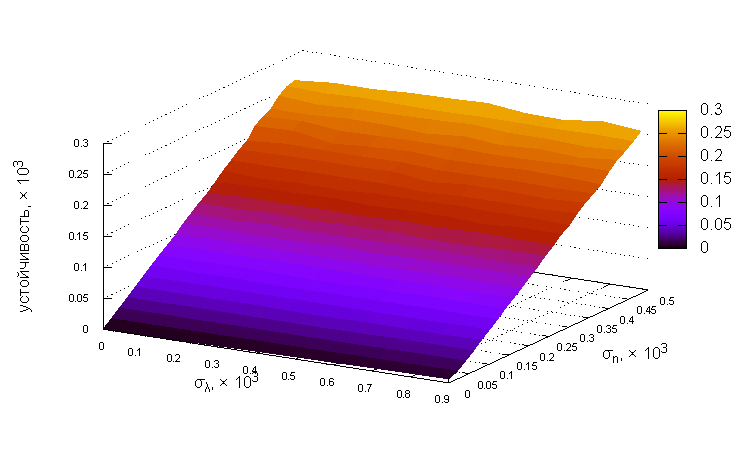
\includegraphics[scale=0.4]{figs/even/p1.txt_coeff0.dat.pdf} & 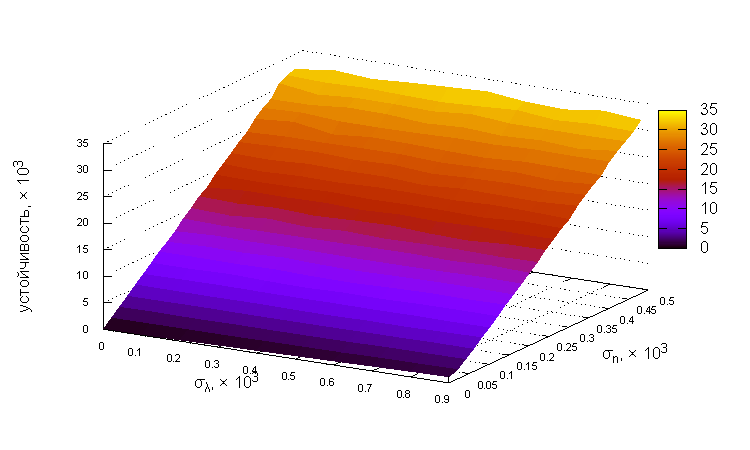
\includegraphics[scale=0.4]{figs/even/p1.txt_coeff1.dat.pdf} & 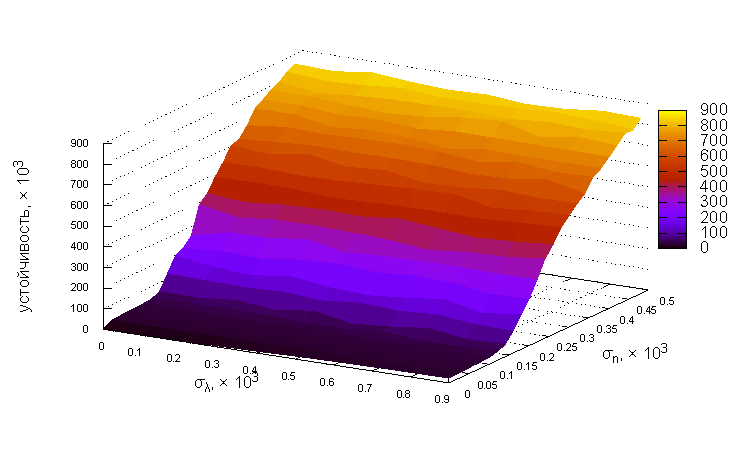
\includegraphics[scale=0.4]{figs/even/p1.txt_coeff2.dat.pdf} \\
	\begin{rotate}{90}Полимер 2\end{rotate} &	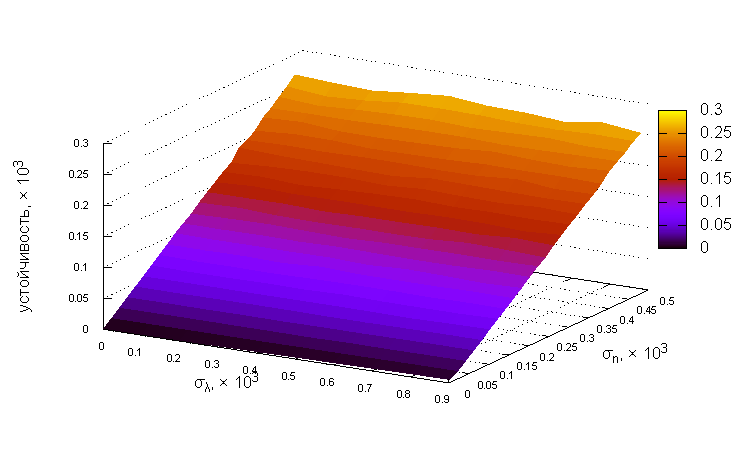
\includegraphics[scale=0.4]{figs/even/p2.txt_coeff0.dat.pdf} & 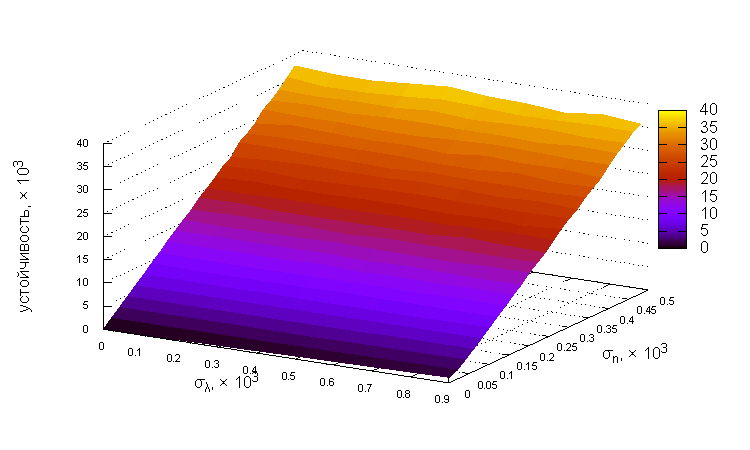
\includegraphics[scale=0.4]{figs/even/p2.txt_coeff1.dat.pdf} & 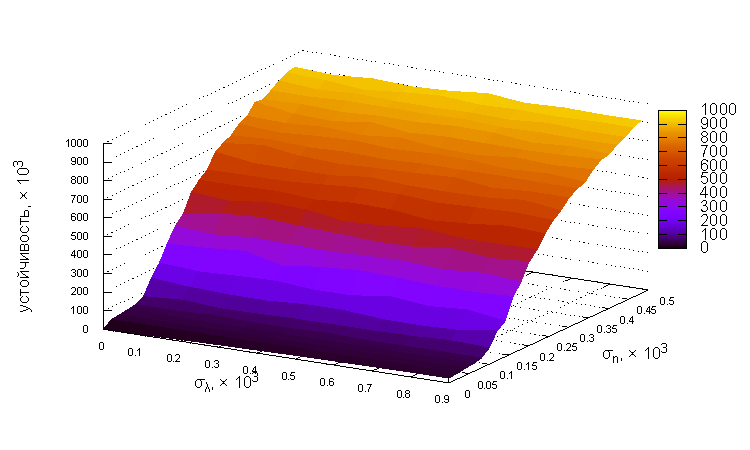
\includegraphics[scale=0.4]{figs/even/p2.txt_coeff2.dat.pdf}
  \end{tabular}
  \caption{Поверхности дисперсии для формулы \eqref{eq:res_0}.}
  \label{tabl:res_even}
\end{table}

\begin{table}[h]
  \centering
  \footnotesize
  \begin{tabular}{| l | c | c | c | c |} \hline
	Полимер		& Коэффициент 1			& Коэффициент 2			& Коэффициент 3			& MSE	\\ \hline
    1			& 1.34946				& 3558.95				& 1924.33				& $2.2 \cdot 10^{-8}$		\\ \hline
    2			& 1.34047				& 3118.84				& 1578.59				& $1.4 \cdot 10^{-8}$		\\ \hline
	Разность	& $6.71 \cdot 10^{-3}$	& $1.41 \cdot 10^{-1}$	& $2.2 \cdot 10^{-1}$	&	\\ \hline
  \end{tabular}
  \caption{Значения коэффициентов для формулы \eqref{eq:res_0} и их относительная разность.}
  \label{tabl:res_even_coeffs}
\end{table}

\begin{table}[h]
  \centering
  \footnotesize
  \begin{tabular}{| l | c | c | c |} \hline
	Коэфф.	& $\frac{\sigma_{\lambda}}{\lambda} = 2 \cdot 10^{-4}; \frac{\sigma_n}{n} = 2 \cdot 10^{-5}$	& $ \frac{\sigma_{\lambda}}{\lambda} = 6 \cdot 10^{-4}; \frac{\sigma_n}{n} = 6 \cdot 10^{-5} $	& $ \frac{\sigma_{\lambda}}{\lambda} = 9 \cdot 10^{-4}; \frac{\sigma_n}{n} = 2 \cdot 10^{-4} $ \\ \hline
	1		& $1.22 \cdot 10^{-5}$																			& $ 3.59 \cdot 10^{-5} $																		& $ 1.19 \cdot 10^{-4} $		\\ \hline
	2		& $1.48 \cdot 10^{-3}$																			& $ 4.38 \cdot 10^{-3} $																		& $ 1.44 \cdot 10^{-2} $		\\ \hline
  \end{tabular}
  \caption{Значения стандартного отклонения для коэффициентов формулы \eqref{eq:res_0} для первого полимера в зависимости от относительных дисперсий.}
  \label{tabl:res_even_stddev}
\end{table}

Из графиков видно, что от шума, накладываемого на значения длины волны, дисперсия значений
первого и второго коэффициентов практически не зависит в достаточно широком диапазоне точности
определения длины волны, представляющем практический интерес. В то же время дисперсия значений
первого коэффициента зависит от дисперсии шума коэффициента преломления практически линейно,
тогда как для второго коэффициента после некоторого характерного значения зависимость становится слабой.

Практическая интерпретация этих результатов~--- при построении прибора для измерения дисперсии
такого типа полимеров в их полосе прозрачности значительное внимание следует уделять точности измерения коэффициента преломления,
тогда как измерения длины волны могут быть неточны вплоть до нескольких нанометров. Кроме того,
предложенный метод прямо указывает, на каких интервалах шума каким будет выигрыш в точности
определения параметров регрессионной модели в зависимости от увеличения точности измерений.

Принципиально важно, что значения стандартного отклонения параметров регрессионной
модели существенно меньше разности между самими значениями этих параметров
(см. таблицы \ref{tabl:res_even_coeffs} и \ref{tabl:res_even_stddev}), что означает, в частности,
что полимеры могут быть различены даже не очень точным рефрактометром.

\paragraph{Стабильность некорректного решения.}

Аналогично исследуем стабильность решения \eqref{eq:res_incorrect}. Приведем только графики
зависимости первых трех коэффициентов, см. таблицу \ref{tabl:res_incorrect}.

\begin{table}[h]
  \centering
  \footnotesize
  \begin{tabular}{l | c c c}
	  & Коэффициент 1 & Коэффициент 2 & Коэффициент 3 \\ \hline
	\begin{rotate}{90}Полимер 1\end{rotate} &	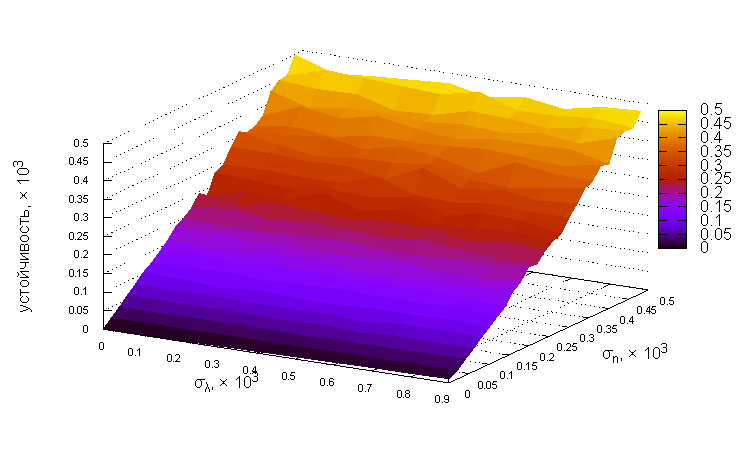
\includegraphics[scale=0.4]{figs/all/p1.txt_coeff0.dat.pdf} & 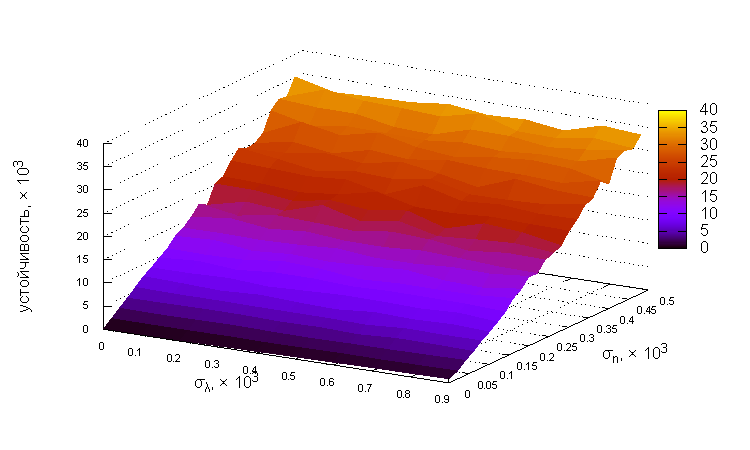
\includegraphics[scale=0.4]{figs/all/p1.txt_coeff1.dat.pdf} & 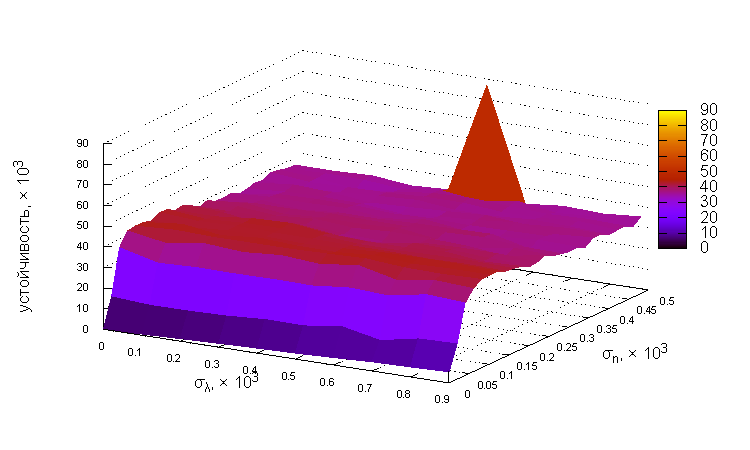
\includegraphics[scale=0.4]{figs/all/p1.txt_coeff2.dat.pdf} \\
	\begin{rotate}{90}Полимер 2\end{rotate} &	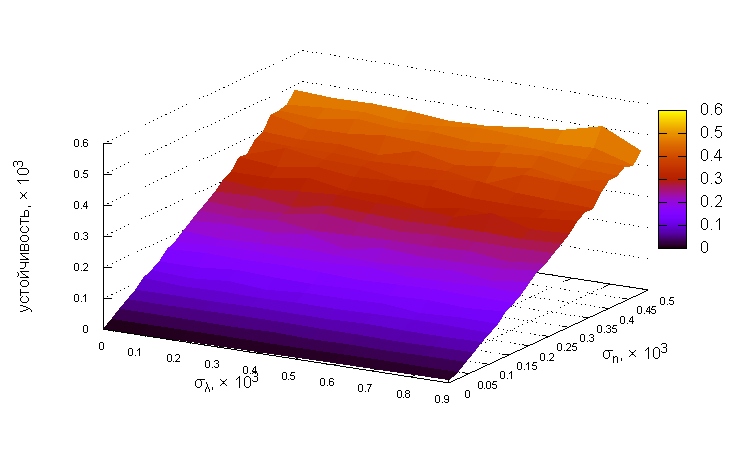
\includegraphics[scale=0.4]{figs/all/p2.txt_coeff0.dat.pdf} & 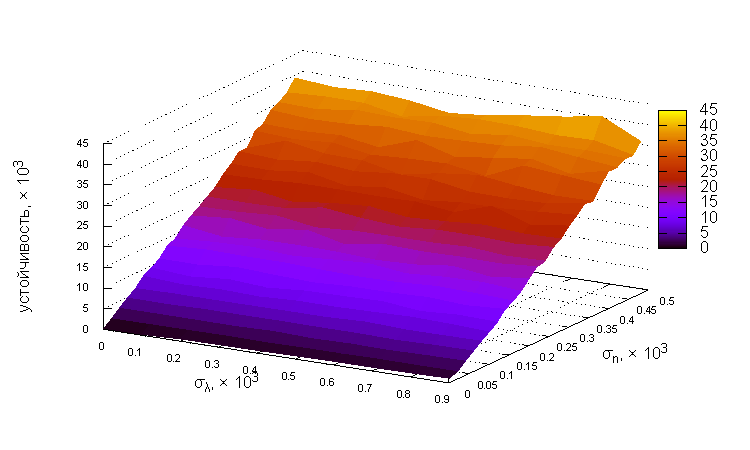
\includegraphics[scale=0.4]{figs/all/p2.txt_coeff1.dat.pdf} & 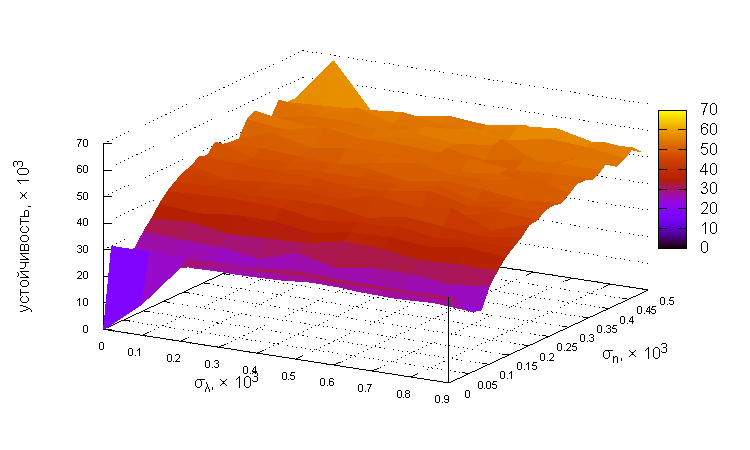
\includegraphics[scale=0.4]{figs/all/p2.txt_coeff2.dat.pdf}
  \end{tabular}
  \caption{Поверхности дисперсии для формулы \eqref{eq:res_incorrect}.}
  \label{tabl:res_incorrect}
\end{table}

Из графиков видно, что в случае формулы \eqref{eq:res_incorrect} стандартное
отклонение соответствующих параметров существенно превышает таковое для
\eqref{eq:res_0}. В частности, второй, третий и четвертый коэффициенты имеют
стандартное отклонение, на порядки превышающее характерные значения самих
коэффициентов.

Данные результаты свидетельствуют о переобучении, и что полученная модель не может быть
использована для надежного приближения экспериментальных данных ввиду большой чувствительности
к шумам.

\begin{comment}
\paragraph{Исследование экспертного предположения.}

Экспертом предположено, что формула также может иметь вид
\begin{equation}
  n(\lambda) = a + \frac{b}{c - \frac{1}{\lambda^2}},
  \label{eq:resonance}
\end{equation}
если измерения находятся вблизи точки резонанса.

Результаты нахождения параметров $a, b$ и $c$ методом Левенберга-Марквардта
приведены в таблице \ref{tabl:resonance_coeffs}.

\begin{table}[h]
  \centering
  \footnotesize
  \begin{tabular}{| c | r | r | r | c |} \hline
	Материал	& $a$							& $b$					& $c$					& MSE						\\ \hline
	1			& $7.333 \cdot 10^{-3}$		& $3.509 \cdot 10^{-4}$	& $1.935 \cdot 10^{-4}$	& $1.7 \cdot 10^{-8}$		\\ \hline
	2			& $1.378$					& $2.352 \cdot 10^{-5}$	& $5.598 \cdot 10^{-5}$	& $3.6 \cdot 10^{-9}$		\\ \hline
  \end{tabular}
  \caption{Значения MSE и коэффициентов формулы \eqref{eq:resonance}.}
  \label{tabl:resonance_coeffs}
\end{table}

\begin{table}[h]
  \centering
  \footnotesize
  \begin{tabular}{l | c c c}
	  & Коэффициент 1 & Коэффициент 2 & Коэффициент 3 \\ \hline
	\begin{rotate}{90}Полимер 1\end{rotate} &	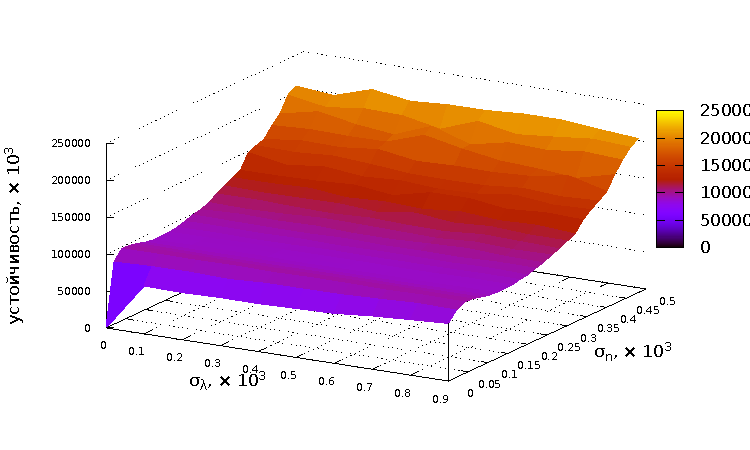
\includegraphics[scale=0.4]{figs/resonance/p1.txt_coeff0.dat.pdf} & 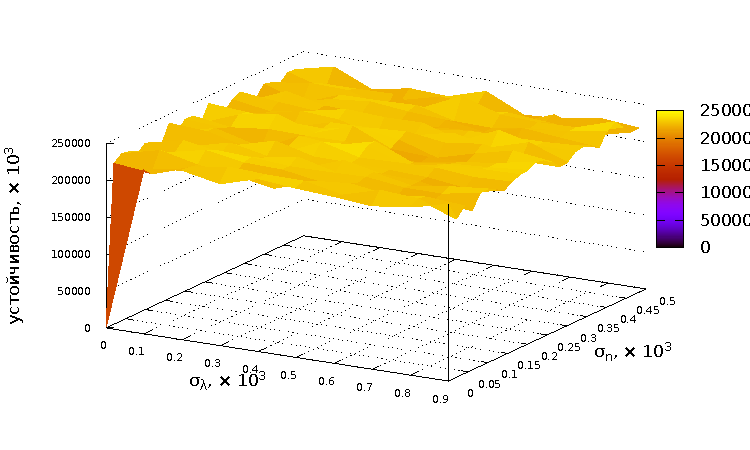
\includegraphics[scale=0.4]{figs/resonance/p1.txt_coeff1.dat.pdf} & 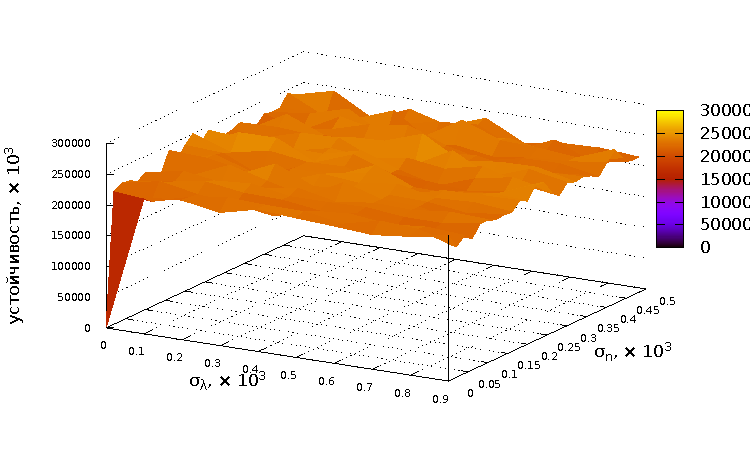
\includegraphics[scale=0.4]{figs/resonance/p1.txt_coeff2.dat.pdf} \\
	\begin{rotate}{90}Полимер 2\end{rotate} &	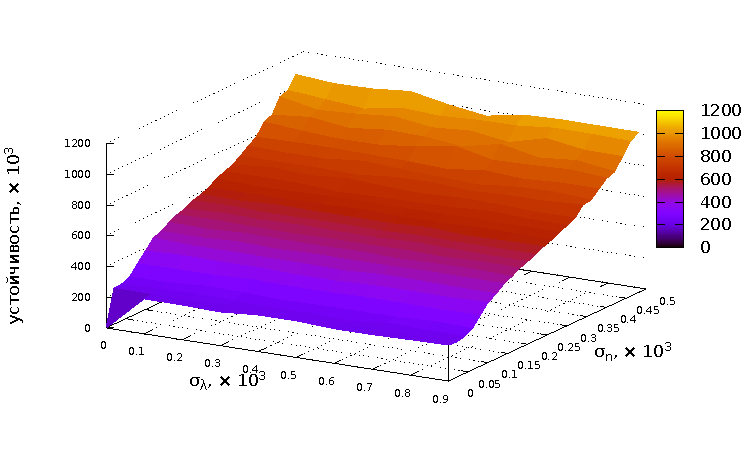
\includegraphics[scale=0.4]{figs/resonance/p2.txt_coeff0.dat.pdf} & 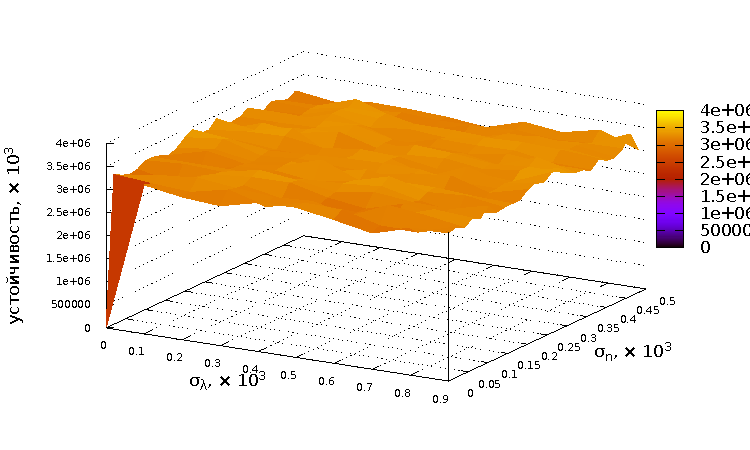
\includegraphics[scale=0.4]{figs/resonance/p2.txt_coeff1.dat.pdf} & 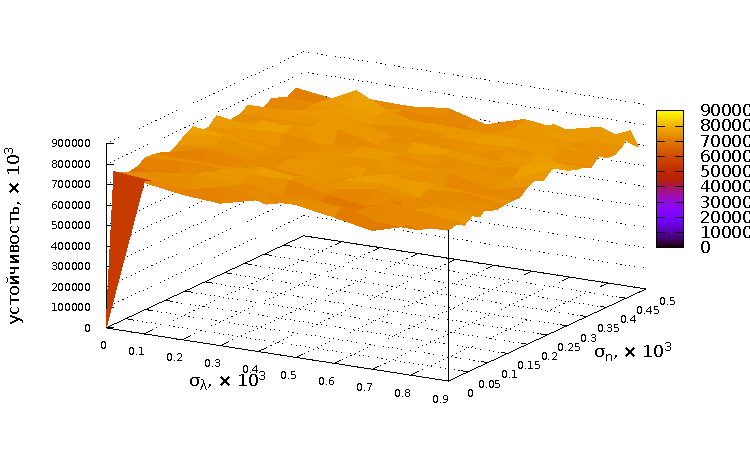
\includegraphics[scale=0.4]{figs/resonance/p2.txt_coeff2.dat.pdf}
  \end{tabular}
  \caption{Поверхности дисперсии для формулы \eqref{eq:resonance}.}
  \label{tabl:res_resonance}
\end{table}

Исследуем стабильность данного решения тем же методом, что и в
предыдущих случаях. Поверхности дисперсии приведены в таблице \ref{tabl:res_resonance}.

Отметим, что характерные дисперсия первого коэффициента на порядки больше, чем
для формулы \eqref{eq:res_0}, что затрудняет различение полимеров в смеси при
достаточно большой погрешности измерения $\lambda$. Кроме того, полученные значения
дисперсий коэффициентов позволяют говорить о, по-видимому, существенной неустойчивости
решения и, как следствие, невозможности его использования в качестве корректной модели.
Поверхности дисперсии также не являются настолько же гладкими, как для формулы
\eqref{eq:res_0}.

Все это позволяет заключить, что, хотя экспериментальные данные хорошо
описываются формулой \eqref{eq:resonance}, они не являются корректными с
экспертно-физической точки зрения.

\end{comment}

\subsubsection{Сходимость к классическому случаю}

Рассмотрим случай, когда зависимость линейна:
\[
  y = ax + b,
\]
и с учетом ошибок измерений представима в виде
\[
  y_i = ax_i + b + \xi_i \mid i \in \{ 1, \dots, n \},
\]
где ошибки $\xi_i$ независимы, $E(\xi_i) = 0; D(\xi_i) = \sigma^2$ \cite{Vatunin05}.
То есть, рассматривается случай независимости ошибки измерения от точки измерения,
при этом независимая переменная измеряется точно.

Перейдем к представлению
\[
  y_i = a(x_i - \overline{x}) + b + \xi_i \mid i \in \{ 1, \dots, n \},
\]
для которого, согласно \cite{Vatunin05}, случайные величины $a$ и $b$ независимы
и нормально распределены, и, кроме того, их дисперсии выражаются известными соотношениями:
\begin{equation}
  \label{eq:classic_da}
  D(a) = \frac{\sigma^2}{\sum_{i = 1}^n (x_i - \overline{x})^2}.
\end{equation}
\begin{equation}
  \label{eq:classic_db}
  D(b) = \frac{\sigma^2}{n}.
\end{equation}

Рассмотрим, насколько результаты предложенного метода отличаются от значений,
полученных согласно \eqref{eq:classic_da} и \eqref{eq:classic_db}. Для этого исследуем
зависимость относительной разности между этими значениями и эмпирическими значениями устойчивости от
числа итераций N:
\[
  \delta_1 = \frac{| \mathbf{T}^N_y(1) - D(a) |}{D(a)},
\]
\[
  \delta_2 = \frac{| \mathbf{T}^N_y(2) - D(b) |}{D(b)}.
\]

Соответствующие графики для функции $y = 2x + 1 + \xi_i$ на интервале $x \in [0; 10]$ при
различном количестве порожденных точек (10 и 50) приведены на рис. \ref{fig:classic_all_0_all}
для значений $D(\xi_i)$, равных 1 и 10. По оси $x$ отложено
число итераций в тысячах (до $10^7$), по $y$~--- значения $\delta_1$ и $\delta_2$.

На рис. $\ref{fig:classic_all_0_500}$ и $\ref{fig:classic_all_1000_all}$ приведены
отдельные графики, соответствующие интервалам от 0 до $5 \cdot 10^5$ итераций и от $10^6$ до
$10^7$ итераций соответственно. Рис. $\ref{fig:classic_all_0_500}$ демонстрирует
сходимость в начале работы алгоритма, в то время как рис. $\ref{fig:classic_all_1000_all}$
показывает характер сходимости при достаточно больших $N$.

Из графиков видно, что значения разности стабилизируются в районе $(1.5 \div 3) \cdot 10^6$
итераций и не демонстрируют явной зависимости от числа точек или дисперсии погрешности.

\begin{figure}[h]
  \centering
  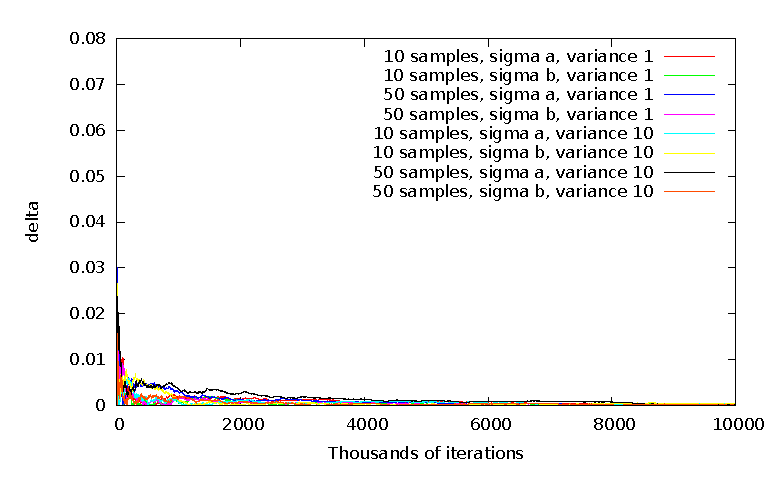
\includegraphics[scale=1.2]{figs/classic/variance_all_0_all.eps}
  \caption{График зависимости $\delta$ от числа итераций (от 0 до $10^7$ итераций).}
  \label{fig:classic_all_0_all}
\end{figure}

\begin{figure}[h]
  \centering
  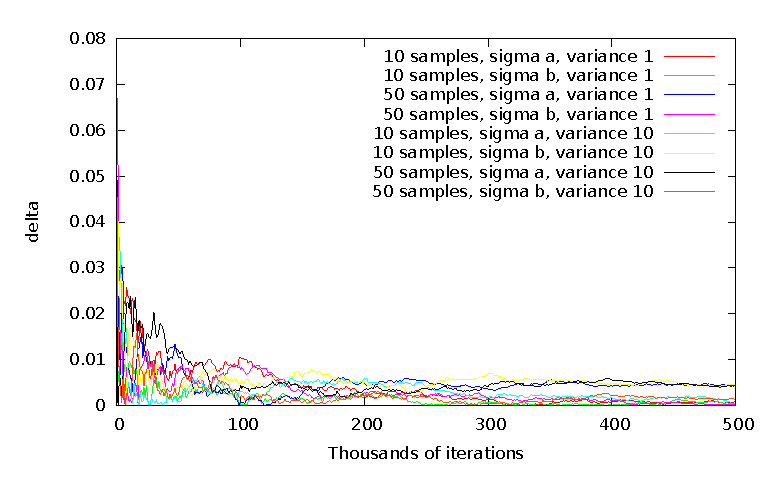
\includegraphics[scale=1.2]{figs/classic/variance_all_0_500.eps}
  \caption{График зависимости $\delta$ от числа итераций (от 0 до $5 \cdot 10^5$ итераций).}
  \label{fig:classic_all_0_500}
\end{figure}

\begin{figure}[h]
  \centering
  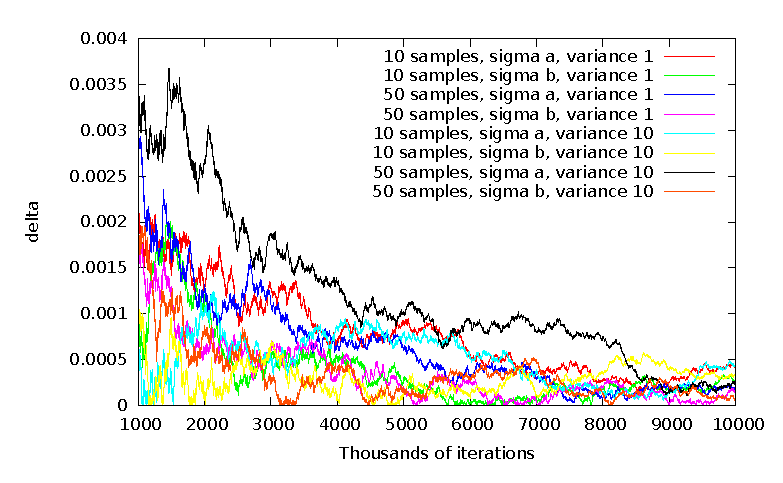
\includegraphics[scale=1.2]{figs/classic/variance_all_1000_all.eps}
  \caption{График зависимости $\delta$ от числа итераций (от $10^6$ до $10^7$ итераций).}
  \label{fig:classic_all_1000_all}
\end{figure}

\section{Заключение}

Предложенный в \cite{Rudoy13} алгоритм позволяет получить интерпретируемую аналитическую
формулу, описывающую зависимость коэффициента преломления среды от длины волны.
Введенный штраф за сложность позволяет избежать переобучения без использования методов
вроде скользящего контроля, и, таким образом, отпадает необходимость в контрольной выборке.

Хотя другие алгоритмы, такие как SVM-регрессия, могут демонстрировать более высокое
качество приближения данных, их результаты неинтерпретируемы и не защищены от переобучения
<<по построению>>, поэтому требуют разделения выборки на обучающую и контрольную. Кроме
того, их структурные параметры так же требуют оценки по методам вроде кросс-валидации.

Предложенный в настоящей работе метод оценки стабильности решения позволяет исследовать вклад различных
членов результирующей суперпозиции и зависимость изменения этих членов от
случайных шумов во входных данных. В частности, в прикладных областях данный метод позволяет
выявить, какие именно элементы признакового описания объектов в генеральной совокупности
наиболее чувствительны к шуму. Кроме того, для корректных с экспертной точки зрения
решений оказывается, что они стабильны, в то время как некорректные результаты нестабильны.

\FloatBarrier

\bibliographystyle{babunsrt-lf}
\bibliography{bibliography}

\end{document}
